%==============================================================================
%  main_applsci_mdpicls.tex — Applied Sciences submission, official mdpi.cls
%
%  Same manuscript as main_applsci.tex, compiled with MDPI's own class.
%  Official bundle lives in ./Definitions/ (from MDPI_template.zip):
%    https://www.mdpi.com/authors/latex
%  Overleaf: set this file as main; TeX Live 202X has enotez/paracol.
%  Local TL2013 may still need a personal texmf for enotez — Overleaf does not.
%==============================================================================
\documentclass[applsci,article,submit,pdftex,oneauthor]{Definitions/mdpi}


%--- mdpi.cls loads paracol, which draws page-building boxes from the same
%--- \@freelist as floats. With 12 floats the stock 18-box list runs out and
%--- LaTeX stops placing floats ("Too many unprocessed floats"). morefloats /
%--- \extrafloats cover this on modern TeX; keep a portable freelist extend
%--- for older kernels and for Overleaf float pressure.
\makeatletter
\newcount\mf@i
\newcommand*\mf@extrafloats[1]{%
  \mf@i=#1\relax
  \loop\ifnum\mf@i>\z@
    \expandafter\newbox\csname mf@box\the\mf@i\endcsname
    \expandafter\@cons\expandafter\@freelist
      \expandafter{\csname mf@box\the\mf@i\endcsname}%
    \advance\mf@i\m@ne
  \repeat}
\mf@extrafloats{80}
\makeatother

\usepackage{pgfplots}
\pgfplotsset{compat=1.16}
\usepgfplotslibrary{groupplots}
\usetikzlibrary{shapes.geometric,arrows.meta,positioning,fit,backgrounds,calc}

%---------------- Okabe-Ito palette (safe under deuteranopia/protanopia) ------
\definecolor{okVermillion}{HTML}{D55E00}
\definecolor{okOrange}{HTML}{E69F00}
\definecolor{okYellow}{HTML}{F0E442}
\definecolor{okGreen}{HTML}{009E73}
\definecolor{okBlue}{HTML}{0072B2}
\definecolor{okSky}{HTML}{56B4E9}
\definecolor{okPurple}{HTML}{CC79A7}
\definecolor{okGold}{HTML}{8C6D31}

%--- DOIs are set in the running font but may break like a URL
\newcommand{\doilink}[1]{\begingroup\urlstyle{same}\url{#1}\endgroup}
\newcommand{\PH}[1]{{\color{red}\textbf{[#1]}}}
% mdpi.cls sets \thesubfigure to (\textbf{a}); sub-panels drawn with pgfplots
% carry the same label, centred beneath the panel rather than above it.
\newcommand{\panel}[2]{{\small(\textbf{#1})~#2}}
\newcolumntype{L}[1]{>{\raggedright\arraybackslash}p{#1}}
\newcolumntype{C}[1]{>{\centering\arraybackslash}p{#1}}
\newcommand{\tnote}[1]{\textsuperscript{#1}}
% MDPI sets table notes flush left beneath the rule, marker separated from the
% note text; \centering is still in force inside the float, hence the reset.
\newcommand{\tabfoot}[1]{\par\vspace{2pt}\begingroup\raggedright\footnotesize
  \noindent #1\par\endgroup}
\newcommand{\tnotedef}[1]{\textsuperscript{#1}\,}

%==============================================================================
%  FRONT MATTER
%==============================================================================
\Title{Metadata-Grounded Large Language Models for Converting Hospital
Statistical Requests into Clinical Data Warehouse Queries}

\TitleCitation{Metadata-Grounded Large Language Models for Converting Hospital
Statistical Requests into Clinical Data Warehouse Queries}

\providecommand{\orcidA}{}

\Author{Shikai Li $^{1,}$*\orcidA{}}

\AuthorNames{Shikai Li}

\AuthorCitation{Li, S.}

% lineage: sole author + Information and Data Management, WCH-SCU (confirmed 2026-07-27)
\address[1]{%
$^{1}$ \quad Department of Information and Data Management, West China Hospital,
Sichuan University, Chengdu 610041, China}

\corres{Correspondence: \PH{corresponding@example.edu}; Tel.: \PH{+86 ...}}

\featuredapplication{The framework converts free-text statistical requests from
clinical departments into executable, provenance-carrying SQL over a hospital
clinical data warehouse, and is deployed on premises so that no patient data
leaves the institution.}

\abstract{Hospital reporting depends on statistical criteria---which timestamp a
case is counted by, which flag defines an indicator---that are
institution-specific and carry no cross-site vocabulary, so free-text requests
from clinical departments still reach a data engineer before they reach the
database. We present a framework that converts such requests into executable
Presto SQL over a three-layer clinical data warehouse, grounding generation in a
metadata knowledge base and verifying every candidate query through syntax,
field, criterion and result checks. Three-stage preprocessing reduced token count
by 56.3\% while preserving statistical semantics. On 398 business terms from 30
reporting tasks, large-language-model mapping reached 52.3\% accuracy against
32.9\% for the rule-based matcher in production ($p<0.001$). A factorial
experiment over 24 tasks, 8 models and 5 prompting strategies produced 960
generation attempts, of which 791 yielded SQL and 274 contained a field or
criterion error. The on-premises qwen2.5:7b model achieved the highest effective
SQL rate, 71.7\% (95\% CI 63.0--79.0), against 60.8\% for gpt-4o, because it
hallucinated less rather than because it generated more. Wrong counting criteria
formed the largest error class at 34.7\%, a failure mode that yields an
executable query and a wrong number, and one that generic schema-linking
taxonomies do not capture.}

\keyword{text-to-SQL; large language models; clinical data warehouse;
hallucination; metadata; statistical criteria; hospital information systems;
retrieval-augmented generation}

%--- journal-assigned fields: the values MDPI's own template ships with -------
\pubvolume{1}
\issuenum{1}
\articlenumber{0}
\pubyear{2026}
\copyrightyear{2026}
\datereceived{}
\daterevised{}
\dateaccepted{}
\datepublished{}
\hreflink{https://doi.org/}

\begin{document}

%==============================================================================
\section{Introduction}
%==============================================================================
Hospital operational reporting is essential for quality control, performance
management, and clinical research, yet it faces a persistent bottleneck in data
retrieval. In our institution, statistical requests submitted by clinical
departments, quality-management offices, and researchers are queued to a small
team of data engineers; over the 2023--2024 period, \PH{XX}\% of requests waited
more than five working days for a first result, and \PH{XX}\% required at least
one round of criterion clarification after delivery. These delays defer
management decisions and, for research requests, extend study timelines and
costs, ultimately limiting how often clinical questions are asked of data that
the institution already owns.

Clinical data warehouses (CDWs) exist to relieve exactly this pressure. Ours follows a three-layer design---data lake (DL), data center (DC), and master data repository (MDR)---in which surgery and anesthesia, blood transfusion, laboratory, pathology, and billing systems are standardized into subject-oriented models queried through Presto \cite{presto2019}. That removes much of the join complexity; internationally the same role is played by shared common data models such as the Observational Medical Outcomes Partnership model \cite{ohdsi2015}, though our reporting is defined against institution-specific indicators rather than a shared vocabulary. However, transforming a free-text
statistical request into a warehouse query remains difficult, because the
request encodes \emph{statistical criteria} rather than data structures. Room-in
time, surgery-completion time, discharge time, and application time are not
interchangeable for counting; ``elective surgery,'' ``unplanned reoperation,''
and ``complication'' are institution-specific definitions whose counting object,
time criterion, and filters must be recovered before any SQL can be written.

Querying structured clinical data directly from natural language has been explored along three lines. The text-to-SQL line of
work has progressed from sequence-to-sequence parsers to schema-linking,
constrained-decoding, and decomposed in-context architectures evaluated on public
benchmarks \cite{zhong2017,yu2018,wang2020,scholak2021,pourreza2023,bird2023,dailsql2024,macsql2024},
and has been carried into the clinical setting through EHR-specific datasets,
generation models trained on them, and reliability-oriented shared tasks that
reward abstention on unanswerable questions
\cite{treqs2020,medts2021,ehrsql2024,ragepi2024,rag2step2025}. A parallel line
converts free-text eligibility criteria into executable cohort queries, from
rule- and parser-based systems to modular query generators
\cite{c2q2019,trialpath2021,leafai2023}. Metadata enrichment with task
decomposition has been applied to clinical registry querying and reported
substantial gains \cite{metaclin2025}. Despite these advances, the automated generation of warehouse
queries from statistical requests faces a critical reliability challenge: LLMs
frequently emit nonexistent column and table identifiers, and---more insidiously
for hospital reporting---assign a plausible but wrong counting criterion, a
failure that produces an executable query and a wrong number.

Recent studies have shown that LLMs, while powerful for natural language
understanding, exhibit substantial error rates when mapping domain terms onto
controlled vocabularies and schemas, and that these rates vary widely with model
and prompt \cite{halluc2024,ragstruct2024,chang2024}. This reliability gap poses a significant barrier to
clinical deployment, because an incorrect criterion mapping does not fail
loudly---it silently changes the denominator of a quality indicator that may be
reported to regulators. Furthermore, hospital deployment adds a constraint that
benchmark studies do not face: patient data may not leave the institution, so
cloud-hosted models can only be used on de-identified metadata, and the choice
between cloud and on-premises models materially affects both accuracy and cost.
Systematic comparisons across models under this constraint remain limited.

This study addresses these challenges through a two-pronged approach. First, we
present an end-to-end automated system that transforms free-text hospital
statistical requests into Presto SQL queries compliant with our three-layer CDW,
validated with real patient data from West China Hospital, Sichuan University. Second, we conduct a
comprehensive evaluation of hallucination patterns across 8 LLMs (both
cloud-based and on-premises) using SynHDW, a de-identified synthetic mirror of
the warehouse, systematically analyzing how model selection and prompt
engineering affect reliability. Our findings reveal that while LLMs can
accelerate query generation from days to minutes, hallucination rates of
20\%--47\% highlight the need for careful model selection and validation
strategies. Surprisingly, our evaluation demonstrated that model scale does not
necessarily correlate with performance, with smaller on-premises models
outperforming larger commercial alternatives in terms of effective SQL
generation. By quantifying these trade-offs and identifying optimal
model--prompt combinations for different reporting scenarios, this work advances
the development of trustworthy and cost-effective AI systems for hospital data
operations.

%==============================================================================
\section{Materials and Methods}
%==============================================================================

\subsection{Study Design}
We conducted a two-phase investigation to develop and validate an automated
system for transforming hospital statistical requests into Presto SQL queries
over a three-layer CDW, followed by systematic analysis of LLM hallucination
patterns. The integrated workflow enables both functional validation and
reliability assessment of LLM-generated queries in real-world reporting
scenarios.

\subsection{Data Sources and Study Population}

\subsubsection{Statistical Request Dataset}
We extracted statistical requests from the reporting ticket system of
West China Hospital, Sichuan University (accessed on 27 July 2026), retaining only tickets that had been
closed with an engineer-authored, criterion-confirmed reference SQL query. We
utilized two distinct datasets: (1) Development Dataset and (2) Validation
Dataset.

First, in the Development Dataset, 30 reporting tasks (10 each from the surgery
and anesthesia, blood transfusion, and laboratory domains) were used exclusively
for metadata dictionary construction and prompt optimization. From these tasks,
we extracted 412 unique business terms for comparative analysis of mapping
approaches between the LLM and RBFM.

Second, in the Validation Dataset, 7 high-usage reporting tasks were selected
based on request frequency over the preceding 24 months (RPT-001, monthly
elective surgery volume by department; RPT-002, unplanned reoperation rate;
RPT-003, postanesthesia care unit [PACU] throughput and delayed-discharge rate;
RPT-004, monthly blood transfusion volume and transfusion-reaction rate;
RPT-005, critical laboratory value notification timeliness; RPT-006, surgical
site infection surveillance denominator; RPT-007, day-surgery share of total
operative volume) for comprehensive system evaluation.

\subsubsection{Clinical Data Infrastructure}
Real-world validation utilized the production CDW of West China Hospital, Sichuan University, a
Presto-based three-layer platform (DL/DC/MDR) integrating 26 source
systems. This comprehensive dataset contains 1,620,000 unique patients with
clinical records spanning from March 2016 to February 2025, exposed
through 398 standardized tables and more than 13,000 columns. All tables
carry a logical-deletion flag, and multi-campus tables carry an organization
code; both must be filtered in every generated query. The study protocol
received approval from the West China Hospital, Sichuan University Institutional Review Board (IRB
No.\ \PH{XXXX-XXXX}).

\subsubsection{Synthetic Data for Hallucination Analysis}
To systematically evaluate hallucination patterns, we employed the Synthetic Hospital Data Warehouse (SynHDW) version 1.0 (generation seed 20251118), a de-identified synthetic mirror of the production warehouse containing 112,680
synthetic patients with visit, surgery, transfusion, and laboratory records from
2019 to 2023. This dataset's limited metadata coverage ($\sim$1680 of the
$>$13,000 production columns) provided an ideal test bed for identifying
hallucination behaviors when models encounter field and criterion mapping
challenges.

\subsection{Statistical Criteria to SQL Transformation Pipeline}
The pipeline transforms free-text statistical requests into Presto-compliant SQL through three modules. Preprocessing runs in three stages: segmentation into individual criteria, preserving Boolean logic and grouping hierarchy; filtration of non-queryable elements such as formatting instructions, deadlines, and narrative justification; and simplification, which standardizes temporal expressions and reduces token count without changing statistical semantics. The information
extraction module identifies seven structured elements from preprocessed text
(Business Terms, Metadata Systems [warehouse schema, metric-criterion
dictionary, historical SQL, exception rules], Field Identifiers, Values,
Attributes, Temporal, and Negation) and then maps each business term to a
warehouse-standardized field and counting criterion using the LLM, following
retrieval-augmented generation practice \cite{lewis2020,finardi2024}. Candidate
tables and columns are recalled by a hybrid sparse--dense scheme combining BM25
\cite{bm252009} with transformer sentence embeddings
\cite{sbert2019,bert2019}; this recall step plays the
role of schema linking, which recent work frames as context-aware bidirectional
retrieval whose central tension is recall versus precision, because aggressive
linking over-includes irrelevant schema elements
\cite{schemalink2025,rslsql2024}. The SQL
generation module creates Presto-compliant queries through iterative refinement
and optimization, emitting a field-provenance record alongside each query. Each
module exchanges data via structured JSON to ensure interoperability throughout
the pipeline. Figure~\ref{fig:arch} shows the pipeline as a whole; Figure S1 of
the Supplementary Materials expands each module into its constituent steps and
names the interfaces between them.

%------------------------------ FIGURE 1 ------------------------------
\begin{figure}[H]
\centering
\vspace{2pt}

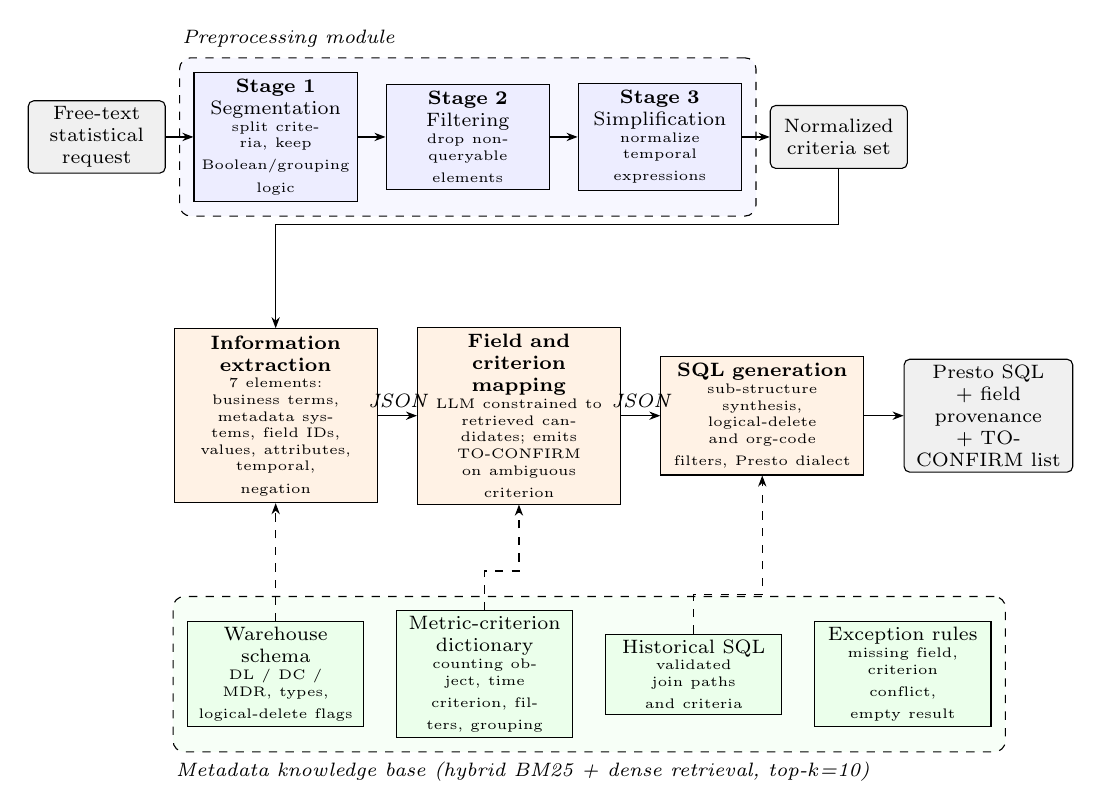
\begin{tikzpicture}[
  font=\scriptsize,
  node distance=3.2mm and 3.5mm,
  io/.style   ={draw,rounded corners=2pt,fill=gray!12,align=center,
                text width=16mm,minimum height=8mm,inner sep=2pt},
  st/.style   ={draw,fill=blue!7,align=center,text width=19mm,
                minimum height=11mm,inner sep=2.5pt},
  mod/.style  ={draw,fill=orange!10,align=center,text width=23mm,
                minimum height=12mm,inner sep=2.5pt},
  kb/.style   ={draw,fill=green!8,align=center,text width=21mm,
                minimum height=7mm,inner sep=2pt},
  lbl/.style  ={font=\scriptsize\itshape,inner sep=1pt},
  >={Stealth[length=4pt]}]

% ---------- Row 1 : preprocessing ----------
\node[io]  (req) {Free-text\\statistical request};
\node[st, right=of req] (s1) {\textbf{Stage 1}\\Segmentation\\{\tiny split criteria, keep\\Boolean/grouping logic}};
\node[st, right=of s1]  (s2) {\textbf{Stage 2}\\Filtering\\{\tiny drop non-queryable\\elements}};
\node[st, right=of s2]  (s3) {\textbf{Stage 3}\\Simplification\\{\tiny normalize temporal\\expressions}};
\node[io, right=of s3]  (norm) {Normalized\\criteria set};

\draw[->] (req)--(s1); \draw[->] (s1)--(s2); \draw[->] (s2)--(s3); \draw[->] (s3)--(norm);

\begin{scope}[on background layer]
\node[draw,dashed,rounded corners,fill=blue!3,inner sep=5pt,fit=(s1)(s2)(s3)] (pre) {};
\end{scope}
\node[lbl,anchor=south west,yshift=0.8mm] at (pre.north west) {Preprocessing module};

% ---------- Row 2 : information extraction ----------
\node[mod, below=16mm of s1.south, anchor=north, text width=24mm] (ie)
  {\textbf{Information extraction}\\{\tiny 7 elements: business terms,\\metadata systems, field IDs,\\values, attributes, temporal,\\negation}};
\node[mod, right=5mm of ie, text width=24mm] (map)
  {\textbf{Field and criterion}\\\textbf{mapping}\\{\tiny LLM constrained to\\retrieved candidates; emits\\TO-CONFIRM on ambiguous\\criterion}};
\node[mod, right=5mm of map, text width=24mm] (gen)
  {\textbf{SQL generation}\\{\tiny sub-structure synthesis,\\logical-delete and org-code\\filters, Presto dialect}};
\node[io, right=5mm of gen, text width=20mm] (out)
  {Presto SQL\\+ field provenance\\+ TO-CONFIRM list};

\draw[->] (norm.south) -- ++(0,-7mm) -| (ie.north);
\draw[->] (ie)--(map); \draw[->] (map)--(gen); \draw[->] (gen)--(out);

% ---------- Row 3 : knowledge base ----------
\node[kb, below=15mm of ie.south, anchor=north] (kb1) {Warehouse schema\\{\tiny DL / DC / MDR, types,\\logical-delete flags}};
\node[kb, right=4mm of kb1] (kb2) {Metric-criterion dictionary\\{\tiny counting object, time\\criterion, filters, grouping}};
\node[kb, right=4mm of kb2] (kb3) {Historical SQL\\{\tiny validated join paths\\and criteria}};
\node[kb, right=4mm of kb3] (kb4) {Exception rules\\{\tiny missing field, criterion\\conflict, empty result}};

\begin{scope}[on background layer]
\node[draw,dashed,rounded corners,fill=green!3,inner sep=5pt,
      fit=(kb1)(kb2)(kb3)(kb4)] (kbx) {};
\end{scope}
\node[lbl,anchor=north west,yshift=-0.8mm] at (kbx.south west)
  {Metadata knowledge base (hybrid BM25 + dense retrieval, top-$k$=10)};

\draw[->,dashed] (kb1.north) -- ++(0,5mm) -| (ie.south);
\draw[->,dashed] (kb2.north) -- ++(0,5mm) -| (map.south);
\draw[->,dashed] (kb3.north) -- ++(0,5mm) -| (gen.south);

% ---------- JSON annotation ----------
\node[lbl,above=0.6mm] at ($(ie.east)!0.5!(map.west)$)  {JSON};
\node[lbl,above=0.6mm] at ($(map.east)!0.5!(gen.west)$) {JSON};

\end{tikzpicture}
\caption{Architecture of the transformation pipeline. A free-text hospital
statistical request passes through three-stage preprocessing, information
extraction, field and criterion mapping, and SQL generation, yielding
Presto-compatible Structured Query Language (SQL) over a three-layer clinical
data warehouse (CDW) together with a field-provenance record and any
TO-CONFIRM items. Solid arrows carry data between modules; dashed arrows
show which part of the metadata knowledge base each module reads. DC: data
center; DL: data lake; JSON: JavaScript Object Notation; LLM: large language
model; MDR: master data repository.}
\label{fig:arch}
\end{figure}

\subsection{Large Language Model Configuration}
We employed gpt-4o (build gpt-4o-2024-08-06) via API and an on-premises deployment of
qwen2.5:7b-instruct served through vLLM, with task-specific prompting strategies
optimized through iterative refinement. Zero-shot prompting was utilized for
straightforward tasks including request segmentation and criterion
classification, which minimized token usage and inference cost. Few-shot
prompting with carefully selected examples enhanced performance for complex
tasks including field and criterion mapping and SQL generation. All prompts
incorporated explicit instructions for Presto dialect compliance, mandatory
logical-deletion and organization-code filtering, and error handling. Decoding
was deterministic (temperature 0, top-$p$ 1) for all models. No patient-level
data were transmitted to any cloud endpoint; cloud models received only
de-identified metadata and synthetic values. Complete prompt templates are
provided in Table S2 of the Supplementary Materials.

\subsection{Comparative Evaluation Framework}

\subsubsection{Business Term Mapping Assessment}
Mapping accuracy was assessed on the 30-task development set (surgery and anesthesia, blood transfusion, laboratory), which spans a wide range of institutional terminology. We compared the LLM with the rule-based field matcher (RBFM) currently deployed in our metadata portal. RBFM is institution-internal and cannot be rerun elsewhere, so we additionally report a externally reproducible reference: selecting, for each business term, the single highest-scoring warehouse field under BM25 over column names and annotations, with no synonym table and no semantic component. While the LLM
performs contextual natural language understanding, RBFM uses string
normalization, Levenshtein distance--based similarity scoring, and a curated
synonym table to identify candidate warehouse fields. In our experiments, RBFM
was run using its production settings, and the top-ranked field based on
similarity score was selected for each input term. Relevant business terms were
extracted from the request text of each task and mapped using both the LLM and
RBFM.

Two clinical data engineers then reviewed both systems' output and fixed the reference by consensus, either choosing the better candidate or assigning a more suitable field themselves.

\subsubsection{SQL Query Validation}
To rigorously evaluate the accuracy and applicability of the generated SQL
queries within the CDW, we conducted an expert-based validation involving two
experts with strong proficiency in both hospital statistical criteria and the
warehouse schema. Generated SQL queries underwent systematic evaluation using 72
predefined evaluation criteria designed to assess three key dimensions: SQL
syntax adherence, warehouse schema compliance, and criteria contextual accuracy.
Each expert independently rated all applicable criteria on a 4-point scale
(1=noncompliant and 4=fully compliant), with final scores calculated as the
average of both ratings.

The evaluation framework was applied differentially based on query content. For
all generated queries, the full set of 72 criteria was used to assess structural
and schema-level accuracy. However, for queries containing business terms from
our prevalidated criterion map, only 18 criteria from the original 72 were
applicable---these specifically evaluated criterion inclusion accuracy and field
identifier correctness. Inter-rater reliability was measured using Cohen kappa,
with discrepancies resolved through consensus discussion.

This expert-driven evaluation allowed for the identification of critical
issues---such as misinterpretation of counting logic, inaccurate temporal
constraints, or improper use of DL-layer tables where a DC-layer aggregate was
required---that automated methods might overlook. As a result, we verified that
the generated SQL queries were not only technically correct but also
statistically meaningful and suitable for use in real-world hospital reporting.
The complete list of evaluation criteria is provided in Table S3 of the
Supplementary Materials.

\subsubsection{Statistical Result Validation}
Building gold-standard cohorts by hand is prohibitive, so we used engineer-authored, criterion-confirmed historical SQL as the reference standard and ran result-set extraction against the production CDW of West China Hospital, Sichuan University. Three reporting tasks qualified---RPT-001, RPT-002, and RPT-005, comprising 28 statistical criteria---because validated reference SQL existed for at least one criterion each. A criterion entered the comparison if it was convertible to a single-statement Presto query and had a validated reference query: elective and emergency surgery volume (RPT-001), unplanned reoperation (RPT-002), and critical laboratory value exposure (RPT-005).

Set similarity between system-generated and reference result sets was quantified
using two complementary set-based metrics: Jaccard index (intersection/union)
and overlap coefficient (intersection/minimum set size). The Jaccard index
provides a symmetric measure of overall similarity, while the overlap
coefficient indicates the extent to which the smaller set is contained within
the larger set, useful for identifying cases of incomplete criterion coverage.
This approach enabled objective assessment of query accuracy without requiring
manual chart review, leveraging established internal reference standards for
scalable validation. Additionally, to demonstrate technical feasibility,
successfully generated SQL queries were executed against SynHDW to assess
retrieval capabilities. Patient counts were recorded for selected tasks where
queries were executed without errors.

\subsection{Experimental Design}\label{sec:expdesign}
Although gpt-4o was used for initial system development due to its strong
performance, the limited metadata coverage in SynHDW provided an opportunity to
systematically compare hallucination patterns across multiple LLMs, informing
optimal model selection for different reporting scenarios. The 24 tasks for the
main study included surgery and anesthesia (7 tasks), blood transfusion (5
tasks), laboratory (5 tasks), medical-record and case-mix (4 tasks), and others
(3 tasks), with complexity levels categorized as simple (10), moderate (9), and
complex (5). We employed a factorial design testing eight LLMs (three
cloud-based: gpt-4o \cite{gpt4}, deepseek-v3 \cite{dsv3}, and claude-3.5-sonnet
\cite{claude35}; five locally deployed: qwen2.5:7b \cite{qwen25}, glm4:9b
\cite{glm4}, llama3:8b \cite{llama3}, deepseek-r1:7b \cite{dsr1}, and phi3
\cite{phi3}) with five prompting
strategies (zero\_shot, structured\_approach, explicit\_uncertainty,
validation\_focused, and error\_aware). The five prompting strategies were
designed to test different approaches to query generation:

\begin{itemize}[leftmargin=1.4em,itemsep=1pt,topsep=2pt]
  \item zero\_shot: Direct query without examples or guidance
  \item structured\_approach: Step-by-step sub-structure decomposition guidance
  \item explicit\_uncertainty: Encouraging TO-CONFIRM use for uncertain criteria
  \item validation\_focused: Emphasizing validation and accuracy requirements
  \item error\_aware: Including SynHDW coverage limits and common pitfalls
\end{itemize}

\noindent Following a pilot phase (6 tasks $\times$ 8 models $\times$ 5
prompts=240 queries) for methodology validation, the main study analyzed 960
queries (24 tasks $\times$ 8 models $\times$ 5 prompts).

\subsection{Hallucination Detection and Classification}
An automated detection system was developed to identify hallucinations in
generated SQL queries. The system validated every table and column identifier
against the SynHDW metadata inventory and verified criterion appropriateness
against the metric-criterion dictionary. For the initial validation phase, we
analyzed SQL generation failures from the seven validation tasks. For the
large-scale model comparison, we developed a five-category hallucination
classification schema ordered by severity. Category A (Critical) comprised
nonexistent table or column identifiers that invalidate query results. Category
B (Major) included valid fields assigned to the wrong counting criterion---for
example, counting a monthly surgical volume by discharge time instead of room-in
time---which yields an executable query and a wrong number. Category C (Major)
captured natural language left in an identifier position, reflecting confusion
between a business term and a column name. Category D (Moderate) consisted of
placeholder values requiring manual intervention. Category E (Minor) encompassed
easily correctable dialect or schema errors, including omission of the mandatory
logical-deletion or organization-code filter. This classification specifically
evaluated model tendencies toward generating inappropriate field and criterion
references, distinct from the initial error analysis.

\subsection{Abstention Quality Assessment}
The pipeline emits a TO-CONFIRM item instead of committing when two or more
counting criteria are defensible for the same indicator. To measure whether that
behaviour is useful rather than merely present, two clinical data engineers
reviewed all 791 generated queries and labelled each for whether the criterion it
encoded was genuinely ambiguous under the institution's indicator definitions.
Against that reference we counted abstentions that were warranted (correct
abstention), abstentions raised on an unambiguous criterion (false abstention),
and ambiguous criteria the system resolved silently instead of asking (missed
abstention). For every missed abstention we further recorded whether the reading
the system chose matched the one the engineers would have chosen.

\subsection{Component Ablation}
To separate the contribution of the three pipeline layers we ran four settings
on the best-performing model, qwen2.5:7b, over the same 24 tasks and 5 prompting
strategies: (A) the bare model receiving only the natural-language request;
(B) A plus the warehouse schema; (C) B plus retrieval over the metadata knowledge
base, the metric-criterion dictionary and historical SQL; and (D) C plus the
four-layer execution-feedback verification, which is the complete system.
Setting D is the qwen2.5:7b condition of the main experiment and is not rerun.
Errors in every setting were classified with the same five-category schema, so
the ablation shows not only how much each layer helps but which error class it
removes.

\subsection{Public Benchmark Reference}
Because the warehouse schema and its counting criteria are institution-private,
absolute performance cannot be compared against published systems on our data.
To give an external reference point we ran the unmodified pipeline, with
qwen2.5:7b, over the development split of the EHRSQL 2024 shared task
\cite{ehrsql2024}, substituting that dataset's schema for our metadata knowledge
base and leaving prompts, retrieval and verification unchanged.

\subsection{Analytical Framework of Model Performance}
Model performance was evaluated across four dimensions. The model performance
dimension compared effective SQL generation rates, hallucination frequencies,
and error distributions across eight LLMs. The prompt strategy dimension
assessed five prompting approaches to identify optimal error minimization
strategies. The subject domain dimension analyzed performance variations across
surgery and anesthesia, blood transfusion, laboratory, medical-record, and
billing concepts. The complexity dimension examined correlations between query
complexity (criteria count, join depth, temporal constraints) and error
occurrence.

\subsection{Statistical Analysis}
Statistical analyses were performed using Python 3.11 (Python Software
Foundation) with the scipy library (version 1.11.4) \cite{scipy2020} and
statsmodels library (version 0.14.0) \cite{statsmodels2010}. For mapping
comparisons between the LLM and RBFM, McNemar's test was applied to paired binary
outcomes \cite{mcnemar1947}. Inter-rater agreement was interpreted according to
conventional benchmarks for the kappa statistic \cite{landis1977}. Three primary performance
metrics were calculated: (1) SQL generation rate as the proportion of tasks
producing syntactically valid SQL, (2) hallucination rate as the proportion of
generated queries containing invalid field identifiers or criterion assignments,
and (3) effective SQL generation rate, calculated as SQL generation rate $\times$ (1--hallucination rate), representing queries both syntactically valid and free from field or criterion hallucinations. This product simplifies exactly to $(\text{generated}-\text{hallucinating})/\text{attempts}$, so the effective rate is a binomial proportion over the fixed 120 attempts per model; we therefore report Wilson score 95\% CIs for it and for the pooled hallucination rate.

Model performance across the eight LLMs was compared using one-way ANOVA
followed by Tukey honestly significant difference (HSD) test for post hoc
pairwise comparisons \cite{tukey1949}. Effect sizes were quantified using Cohen $d$ to assess the
practical significance of differences between prompting strategies. $\chi^2$
tests evaluated the distribution of hallucination types across models. Multiple
linear regression analysis identified predictors of hallucination rates, with
model type, prompt strategy, and query complexity as independent variables;
model fit was assessed using $R^2$. All statistical tests employed $\alpha$=.05. Family-wise error across the pairwise model contrasts is controlled by the Tukey HSD procedure itself, so no further Bonferroni adjustment is layered on those comparisons; Bonferroni correction is applied only to the post hoc cell-wise comparisons following the $\chi^2$ test of the hallucination-type distribution.

\subsection{Ethical Considerations}
This study protocol was reviewed and approved by the Institutional Review Board
of West China Hospital, Sichuan University (IRB No.\ \PH{XXXX-XXXX}). As this study did not involve
prospective human participants, informed consent was waived. All data used in
the study were de-identified prior to analysis, no individual-level identifiable
information was accessed, and all model inference on real data was performed on
premises so that patient data never left the institution.

\subsection{Data and Code Availability}
Source code for the pipeline and the hallucination detector, together with the
SynHDW generator and its schema manifest, is available from the corresponding
author upon reasonable request, subject to institutional data-governance rules.
De-identified metadata schemas, the metric-criterion dictionary, and the
evaluation task set are likewise available upon request with appropriate data
use agreements. Patient-level warehouse data cannot be shared. Deployment and
reproduction notes are provided with the code package on request.

%==============================================================================
\section{Results}
%==============================================================================

\subsection{Preprocessing and Statistical Criteria Extraction}
Analysis of the seven validation tasks revealed substantial heterogeneity in
request complexity, ranging from 9 to 22 criteria per task (13.9$\pm$4.2). The
three-stage preprocessing pipeline systematically reduced linguistic complexity
while preserving statistical semantics (Figure~\ref{fig:preproc}). Initial
segmentation achieved modest token reduction (370.4$\pm$63.5) while maintaining
structural integrity. Subsequent filtering of non-queryable request elements
reduced both criteria count (11.4$\pm$3.5) and token count (329.0$\pm$56.5).
Final simplification yielded 9.4$\pm$3.0 criteria with 161.9$\pm$27.9 tokens per
task, representing a 56.3\% overall token reduction.

%------------------------------ FIGURE 2 ------------------------------
\begin{figure}[H]
\centering
\vspace{2pt}

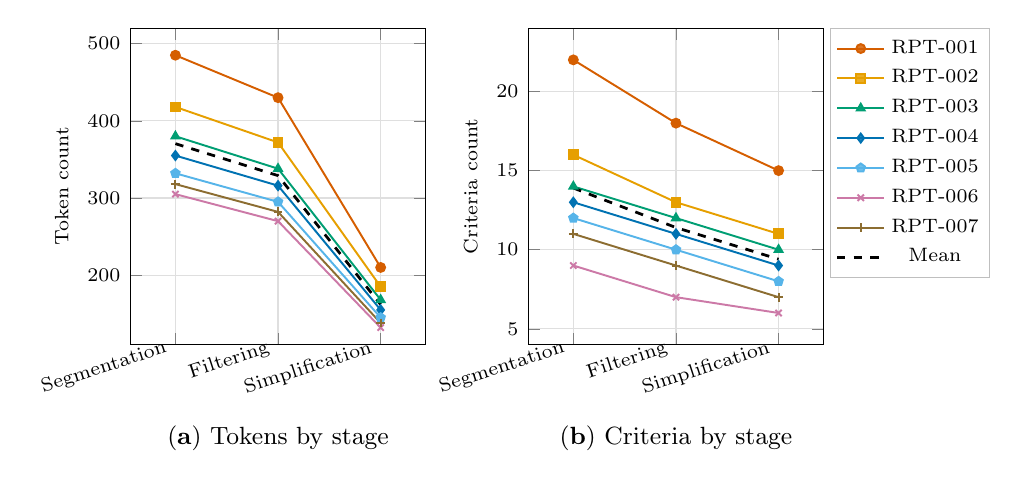
\begin{tikzpicture}
\begin{groupplot}[
  group style={group size=2 by 1, horizontal sep=13mm},
  width=0.44\linewidth, height=5.6cm,
  /tikz/font=\scriptsize,
  symbolic x coords={Segmentation,Filtering,Simplification},
  xtick=data,
  x tick label style={rotate=18,anchor=east},
  enlarge x limits=0.22,
  grid=major, grid style={gray!25},
  legend style={font=\scriptsize,draw=gray!50,fill=white,fill opacity=0.85,
                text opacity=1,at={(1.02,1.0)},anchor=north west,
                row sep=0.5pt,inner sep=2pt},
  every axis plot/.append style={mark size=1.6pt,line width=0.7pt},
  % seven distinct CVD-safe hues, one per task (default cycle reused blue/red)
  cycle list={{okVermillion},{okOrange},{okGreen},{okBlue},{okSky},{okPurple},{okGold}},
]

%------------- Panel A : tokens -------------
\nextgroupplot[ylabel={Token count},ymin=110,ymax=520,
               xlabel={\panel{a}{Tokens by stage}},
               xlabel style={yshift=-1mm}]
\addplot+[mark=*]        coordinates {(Segmentation,485)(Filtering,430)(Simplification,210)};
\addplot+[mark=square*]  coordinates {(Segmentation,418)(Filtering,372)(Simplification,185)};
\addplot+[mark=triangle*]coordinates {(Segmentation,380)(Filtering,338)(Simplification,168)};
\addplot+[mark=diamond*] coordinates {(Segmentation,355)(Filtering,316)(Simplification,155)};
\addplot+[mark=pentagon*]coordinates {(Segmentation,332)(Filtering,295)(Simplification,145)};
\addplot+[mark=x]        coordinates {(Segmentation,305)(Filtering,270)(Simplification,132)};
\addplot+[mark=+]        coordinates {(Segmentation,318)(Filtering,282)(Simplification,138)};
\addplot[black,dashed,line width=1pt,mark=none]
  coordinates {(Segmentation,370.4)(Filtering,329.0)(Simplification,161.9)};

%------------- Panel B : criteria -------------
\nextgroupplot[ylabel={Criteria count},ymin=4,ymax=24,
               xlabel={\panel{b}{Criteria by stage}},
               xlabel style={yshift=-1mm}]
\addplot+[mark=*]        coordinates {(Segmentation,22)(Filtering,18)(Simplification,15)};
\addlegendentry{RPT-001}
\addplot+[mark=square*]  coordinates {(Segmentation,16)(Filtering,13)(Simplification,11)};
\addlegendentry{RPT-002}
\addplot+[mark=triangle*]coordinates {(Segmentation,14)(Filtering,12)(Simplification,10)};
\addlegendentry{RPT-003}
\addplot+[mark=diamond*] coordinates {(Segmentation,13)(Filtering,11)(Simplification,9)};
\addlegendentry{RPT-004}
\addplot+[mark=pentagon*]coordinates {(Segmentation,12)(Filtering,10)(Simplification,8)};
\addlegendentry{RPT-005}
\addplot+[mark=x]        coordinates {(Segmentation,9)(Filtering,7)(Simplification,6)};
\addlegendentry{RPT-006}
\addplot+[mark=+]        coordinates {(Segmentation,11)(Filtering,9)(Simplification,7)};
\addlegendentry{RPT-007}
\addplot[black,dashed,line width=1pt,mark=none]
  coordinates {(Segmentation,13.9)(Filtering,11.4)(Simplification,9.4)};
\addlegendentry{Mean}
\end{groupplot}
\end{tikzpicture}
\caption{Progressive reduction in token count and criteria through preprocessing
stages. (\textbf{a}) Token count changes across segmentation, filtering, and
simplification stages for seven validation tasks. (\textbf{b}) Corresponding changes in
criteria count. Tasks shown are as follows: RPT-001 (monthly elective surgery
volume by department), RPT-002 (unplanned reoperation rate), RPT-003
(postanesthesia care unit throughput and delayed-discharge rate), RPT-004
(monthly blood transfusion volume and transfusion-reaction rate), RPT-005
(critical laboratory value notification timeliness), RPT-006 (surgical site
infection surveillance denominator), RPT-007 (day-surgery share of total
operative volume). Dashed black line indicates the mean across tasks.}
\label{fig:preproc}
\end{figure}

This preprocessing identified 66 statistical criteria suitable for automated
query generation. Information extraction from these 67 preprocessed criteria
yielded 158 unique business terms successfully mapped to warehouse-compatible
elements. Domain distribution analysis revealed that surgery and anesthesia
concepts comprised the predominant category (n=58, 36.7\%), followed by registration and visit (n=27, 17.1\%), diagnosis and medical record (n=23, 14.6\%), laboratory (n=17, 10.8\%), blood transfusion (n=13, 8.2\%), fee and billing (n=10, 6.3\%), staff and organization (n=6, 3.8\%), and ward and bed (n=4, 2.5\%) domains (Table~\ref{tab:domains}). Term frequency analysis
identified time-criterion terms as the most prevalent. ``Operation room-in
time'' appeared in all 7 tasks (100.0\%; 12 mentions). Other frequent terms
included ``discharge date'' (6/7 tasks, 85.7\%; 9 mentions), ``department'' (5/7 tasks, 71.4\%; 8 mentions), ``elective surgery'' (4/7 tasks, 57.1\%; 6 mentions), ``unplanned reoperation'' (3/7 tasks, 42.9\%; 4 mentions), ``ASA
physical status classification'' (2/7 tasks, 28.6\%; 3 mentions), ``transfusion
reaction'' (2/7 tasks, 28.6\%; 3 mentions), and ``complication'' (2/7 tasks, 28.6\%; 2 mentions), as shown in Table~\ref{tab:terms}. Percentages are
calculated based on the number of tasks in which the term appeared, and mentions
indicate the number of criteria within tasks in which the term appeared.

%------------------------------ TABLE 1 ------------------------------
\begin{table}[H]
\caption{Distribution of extracted business terms by clinical data warehouse
(CDW)\tnote{1} subject domain.}
\label{tab:domains}
\centering
\footnotesize
\begin{tabular*}{\linewidth}{@{\extracolsep{\fill}}ll@{}}
\toprule
Domains & Count (n=158), n (\%)\\
\midrule
Surgery and anesthesia        & 58 (36.7)\\
Registration and visit        & 27 (17.1)\\
Diagnosis and medical record  & 23 (14.6)\\
Laboratory                    & 17 (10.8)\\
Blood transfusion             & 13 (8.2)\\
Fee and billing               & 10 (6.3)\\
Staff and organization        & 6 (3.8)\\
Ward and bed                  & 4 (2.5)\\
\bottomrule
\end{tabular*}
\tabfoot{\tnotedef{1}CDW: clinical data warehouse.}
\end{table}

%------------------------------ TABLE 2 ------------------------------
\begin{table}[H]
\caption{Ten most frequently occurring business terms across all tasks.}
\label{tab:terms}
\centering
\footnotesize
\begin{tabular*}{\linewidth}{@{\extracolsep{\fill}}lll@{}}
\toprule
Business terms & Tasks (n=7), n (\%) & Mentions (criterion), n\\
\midrule
Operation room-in time                 & 7 (100.0) & 12\\
Discharge date                         & 6 (85.7)  & 9\\
Department                             & 5 (71.4)  & 8\\
Elective surgery                       & 4 (57.1)  & 6\\
Unplanned reoperation                  & 3 (42.9)  & 4\\
ASA\tnote{1} physical status classification & 2 (28.6) & 3\\
Transfusion reaction                   & 2 (28.6)  & 3\\
Complication                           & 2 (28.6)  & 2\\
PACU\tnote{2} discharge time           & 1 (14.3)  & 2\\
Critical laboratory value              & 1 (14.3)  & 1\\
\bottomrule
\end{tabular*}
\tabfoot{\tnotedef{1}ASA: American Society of Anesthesiologists.\\
\tnotedef{2}PACU: postanesthesia care unit.}
\end{table}

\subsection{Comparative Performance of Mapping Approaches}
Evaluation of mapping accuracy demonstrated the LLM's superior performance
compared to RBFM across 398 business terms extracted from the 30 development
tasks. The LLM achieved an overall accuracy of 52.3\% (208/398) versus RBFM's 32.9\% (131/398), a statistically significant difference ($P<.001$, McNemar's
test). Domain-stratified analysis revealed the LLM's highest accuracy in the
surgery and anesthesia domain (70.7\%, 58/82) and lowest in the laboratory domain (34.5\%, 29/84), suggesting particular challenges with test-item concepts
requiring numeric threshold and unit interpretation.

The BM25-only reference reached 24.4\% (97/398), below RBFM, which is expected since RBFM adds a curated synonym table on top of string similarity; it is reported so that readers outside the institution have a baseline they can reconstruct. Notably, among the 267 terms that RBFM misclassified, the LLM correctly mapped 72 (27.0\%), demonstrating superior contextual understanding. For instance, RBFM
incorrectly mapped ``operation room-in time'' to the admission timestamp on the
registration table---a lexically close but semantically different field---while
the LLM correctly identified the room-in timestamp on the anesthesia record.
This pattern of improved semantic interpretation was consistent across
multiword, criterion-bearing terms.

\subsection{SQL Query Generation Quality and Expert Validation}
Two domain experts independently evaluated SQL queries generated from the seven
validation tasks using 72 predefined criteria across three dimensions: SQL
syntax adherence, warehouse schema compliance, and criteria contextual accuracy
(inter-rater reliability: Cohen $\kappa$=0.79). Each criterion was rated on a
4-point scale (1=noncompliant and 4=fully compliant). SQL syntax adherence
achieved high scores from expert reviewers (3.92$\pm$0.16) and near-ceiling LLM self-evaluation (4.00$\pm$0.00), confirming robust syntactic generation
capabilities. Warehouse schema compliance similarly demonstrated strong
performance (expert: 3.78$\pm$0.28, LLM: 3.98$\pm$0.06), indicating successful
adaptation to the layered table structures and their join paths.

However, criteria contextual accuracy exhibited greater variability and lower
absolute scores (expert: 2.96$\pm$0.48, LLM: 3.41$\pm$0.36), with the 0.45-point difference suggesting systematic LLM overconfidence in criterion
interpretation ($P$=.021, paired $t$ test). This divergence was most pronounced
for criteria involving temporal choices or multicondition counting logic.

Among the total queries evaluated, 24 contained prevalidated criteria from our
development dataset, enabling additional validation of mapping accuracy. For
these queries, criterion inclusion accuracy averaged 3.22$\pm$0.44 (expert) versus 3.45$\pm$0.33 (LLM), while field identifier correctness achieved higher scores of 3.68$\pm$0.29 (expert) versus 3.98$\pm$0.06 (LLM).
The near-ceiling LLM score for field identifier correctness reflects its consistent
ability to generate syntactically valid identifiers, though not necessarily
criterion-appropriate ones.

\subsection{Statistical Result Retrieval Performance}
Validation using engineer-certified reference SQL revealed that performance
strongly correlated with criterion complexity (Table~\ref{tab:retrieval}). For
the three evaluated tasks (RPT-001, RPT-002, and RPT-005), we assessed four
distinct statistical criteria that had available reference standards. The query
for elective surgery volume (RPT-001) demonstrated high retrieval accuracy,
achieving a Jaccard index of 0.79 and a perfect overlap coefficient of 1.0,
indicating that the system-generated result set closely matched the reference
set. In contrast, emergency surgery volume showed a very low Jaccard index of 0.08 despite an overlap coefficient of 1.0, suggesting that while the retrieved
cases were all contained in the reference set, a large portion of the reference
cases was not captured---traced to the model filtering on a single emergency
flag rather than the institution's two-flag definition. The unplanned
reoperation criterion (RPT-002) resulted in complete retrieval failure, with
both the Jaccard index and overlap coefficient equal to 0, indicating that no
matching cases were retrieved. This reflects the system's selection of a
structurally plausible planning flag that is unpopulated throughout the
warehouse, rather than the reoperation marker actually used by the surgical
application table---a failure mode invisible to syntax and schema checking. The
critical laboratory value exposure criterion (RPT-005) achieved moderate
performance, with a Jaccard index of 0.27 and an overlap coefficient of 0.48,
reflecting partial mapping success for an indicator represented by a mix of
numeric thresholds and notification records.

%------------------------------ TABLE 3 ------------------------------
\begin{table}[H]
\caption{Comparison of result-set retrieval between system-generated queries and
validated reference SQL\tnote{1}.}
\label{tab:retrieval}
\centering
\footnotesize
\begin{tabular*}{\linewidth}{@{\extracolsep{\fill}}llll@{}}
\toprule
Task ID & Simplified criterion & Jaccard similarity & Overlap coefficient\\
\midrule
RPT-002 & Unplanned reoperation                & 0    & 0\\
RPT-001 & Emergency surgery volume             & 0.08 & 1.0\\
        & Elective surgery volume              & 0.79 & 1.0\\
RPT-005 & Critical laboratory value exposure   & 0.27 & 0.48\\
\bottomrule
\end{tabular*}
\tabfoot{\tnotedef{1}SQL: Structured Query Language.}
\end{table}

Across these four criteria the system performed well on the one well-defined, single-criterion indicator (elective surgery volume) and poorly on the three whose definitions are compound, institution-specific, or dependent on a sparsely populated field (emergency surgery volume, unplanned reoperation, and critical laboratory value exposure). Four criteria drawn from three tasks cannot establish that this contrast generalizes; we report it as a case series that motivates the error analysis rather than as an estimate of where the system succeeds. Improvements
in criterion dictionary coverage and field-population profiling may be necessary
to enhance retrieval for more complex statistical criteria.

\subsection{Large-Scale Model Comparison and Hallucination Analysis}
To systematically evaluate hallucination patterns across multiple LLMs, we
conducted a separate large-scale experiment using SynHDW, analyzing 960 SQL
generation attempts (24 reporting tasks $\times$ 8 models $\times$ 5 prompting
strategies), distinct from our initial validation study. Analysis of 960 SQL generation attempts revealed significant heterogeneity in model performance ($F_{7,783}$=4.18, $P<.001$). One caveat applies to that omnibus test: phi3 produced SQL for only 18.3\% of attempts, and including a group that degenerate inflates the between-group variance. Hallucination rates ranged from 20.4\%
(n=22/108) to 47.1\% (n=49/104) among models achieving $>$80\% SQL generation
success. The overall hallucination rate was 34.6\% (n=274/791 generated queries) (95\% CI 31.4\%--38.0\%). Because this pools models whose generation rates differ by a factor of five, we also report it restricted to the seven models that generated SQL for more than 80\% of attempts: 35.4\% (n=272/769; 95\% CI 32.1\%--38.8\%). The two estimates differ by 0.7 percentage points, so the pooled figure is not an artifact of including the degenerate model. Variation was substantial in both generation capability and accuracy across models
(Figure~\ref{fig:models} and Table~\ref{tab:modelperf}).

%------------------------------ FIGURE 3 ------------------------------
\begin{figure}[H]
\begin{adjustwidth}{-\extralength}{0cm}
\centering
\vspace{2pt}

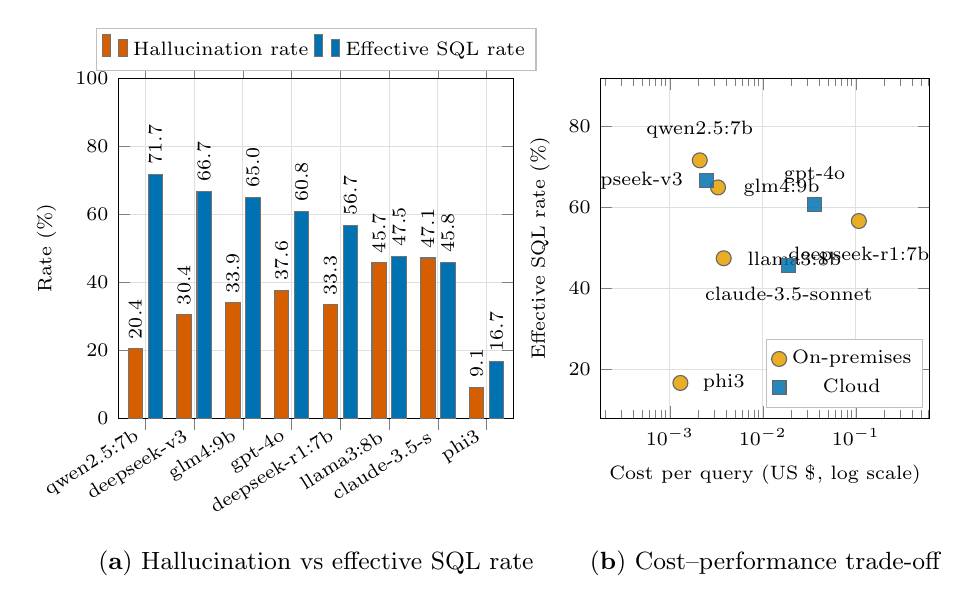
\begin{tikzpicture}
%------------- Panel A -------------
\begin{scope}[local bounding box=bbA]
\begin{axis}[
  name=panelA,
  width=0.545\linewidth, height=5.9cm, font=\scriptsize,
  ybar, bar width=5.2pt,
  symbolic x coords={qwen2.5:7b,deepseek-v3,glm4:9b,gpt-4o,deepseek-r1:7b,
                     llama3:8b,claude-3.5-s,phi3},
  xtick=data, x tick label style={rotate=32,anchor=east,font=\scriptsize},
  ymin=0, ymax=100, ylabel={Rate (\%)},
  grid=major, grid style={gray!25},
  legend style={font=\scriptsize,at={(0.5,1.02)},anchor=south,legend columns=2,
                draw=gray!50,inner sep=2pt},
  enlarge x limits=0.08,
  nodes near coords={\pgfmathprintnumber[fixed,fixed zerofill,precision=1]{\pgfplotspointmeta}},
  every node near coord/.append style={font=\scriptsize,rotate=90,anchor=west},
]
\addplot[fill=okVermillion,draw=black!55] coordinates {
  (qwen2.5:7b,20.4) (deepseek-v3,30.4) (glm4:9b,33.9) (gpt-4o,37.6)
  (deepseek-r1:7b,33.3) (llama3:8b,45.7) (claude-3.5-s,47.1) (phi3,9.1)};
\addlegendentry{Hallucination rate}
\addplot[fill=okBlue,draw=black!55] coordinates {
  (qwen2.5:7b,71.7) (deepseek-v3,66.7) (glm4:9b,65.0) (gpt-4o,60.8)
  (deepseek-r1:7b,56.7) (llama3:8b,47.5) (claude-3.5-s,45.8) (phi3,16.7)};
\addlegendentry{Effective SQL rate}
\end{axis}
\end{scope}

%------------- Panel B -------------
\begin{scope}[local bounding box=bbB]
\begin{axis}[
  name=panelB, at={($(panelA.east)+(11mm,0)$)}, anchor=west,
  width=0.475\linewidth, height=5.9cm, font=\scriptsize,
  xmode=log, log basis x=10,
  xlabel={Cost per query (US \$, log scale)},
  ylabel={Effective SQL rate (\%)},
  xmin=0.00018, xmax=0.62, ymin=8, ymax=92,
  grid=major, grid style={gray!25},
  legend style={font=\scriptsize,at={(0.98,0.03)},anchor=south east,draw=gray!50,inner sep=2pt},
]
% on-premises models (orange)
\addplot[only marks, mark=*, mark size=2.7pt,
         mark options={draw=black!60,fill=okOrange,fill opacity=0.85}]
  table[x=x,y=y] {
x        y     sz
0.0021   71.7  6.5
0.0033   65.0  6.0
0.1078   56.7  5.3
0.0038   47.5  4.6
0.0013   16.7  2.1
};
\addlegendentry{On-premises}
% cloud models (blue)
\addplot[only marks, mark=square*, mark size=2.5pt,
         mark options={draw=black!60,fill=okBlue,fill opacity=0.85}]
  table[x=x,y=y] {
x        y     sz
0.0025   66.7  6.1
0.0190   45.8  4.5
0.0360   60.8  5.7
};
\addlegendentry{Cloud}
% annotations (placed to avoid mutual overlap and axis-edge clipping)
\node[font=\scriptsize,anchor=south,yshift=1.6mm]      at (axis cs:0.0021,71.7) {qwen2.5:7b};
\node[font=\scriptsize,anchor=east,xshift=-1.8mm]      at (axis cs:0.0025,66.7) {deepseek-v3};
\node[font=\scriptsize,anchor=south,yshift=1.4mm]      at (axis cs:0.0360,60.8) {gpt-4o};
\node[font=\scriptsize,anchor=west,xshift=2.0mm]       at (axis cs:0.0033,65.0) {glm4:9b};
\node[font=\scriptsize,anchor=north,yshift=-2.0mm]     at (axis cs:0.1078,56.7) {deepseek-r1:7b};
\node[font=\scriptsize,anchor=west,xshift=1.8mm]       at (axis cs:0.0038,47.5) {llama3:8b};
\node[font=\scriptsize,anchor=north,yshift=-1.6mm]     at (axis cs:0.0190,45.8) {claude-3.5-sonnet};
\node[font=\scriptsize,anchor=west,xshift=1.6mm]       at (axis cs:0.0013,16.7) {phi3};
\end{axis}
\end{scope}
% MDPI panel labels: centred under each panel, on one common baseline
\coordinate (lbly) at ([yshift=-1.4mm]current bounding box.south);
\node[anchor=north] at (panelA.center |- lbly) {\panel{a}{Hallucination vs effective SQL rate}};
\node[anchor=north] at (panelB.center |- lbly) {\panel{b}{Cost--performance trade-off}};
\end{tikzpicture}
\caption{Performance of the eight large language models on clinical data
warehouse (CDW) Structured Query Language (SQL) generation. (\textbf{a})
Hallucination rate and effective SQL rate by model, over 120 attempts each.
(\textbf{b}) Cost per query against effective SQL rate; cloud models are
drawn as blue squares, on-premises models as orange circles. On-premises models incur no per-query API charge;
they are plotted at their amortized cost, computed as inference time $\times$
US~\$0.28 per GPU-hour under the institution's 3-year hardware amortization.}
\label{fig:models}
\end{adjustwidth}
\end{figure}

%------------------------------ TABLE 4 ------------------------------
\begin{table}[H]
\begin{adjustwidth}{-\extralength}{0cm}
\caption{Model performance summary.}
\label{tab:modelperf}
\centering
\footnotesize
\setlength{\tabcolsep}{4pt}
\begin{tabular*}{\linewidth}{@{\extracolsep{\fill}}L{3.3cm}L{2.0cm}L{2.0cm}L{2.1cm}L{2.0cm}L{2.5cm}L{2.0cm}@{}}
\toprule
Model & Architec\-ture & SQL\tnote{1} genera\-tion (\%) & Halluci\-nation (\%)\tnote{2}
      & Effec\-tive SQL (\%)\tnote{3} & Time (s)\tnote{4} & Cost (US \$)/Query\\
\midrule
qwen2.5:7b        & On-premises & 90.0  & 20.4          & 71.7 & 27.3$\pm$6.4      & 0.000\\
deepseek-v3       & Cloud       & 95.8  & 30.4          & 66.7 & 7.6$\pm$1.9       & 0.003\\
glm4:9b           & On-premises & 98.3  & 33.9          & 65.0 & 41.8$\pm$10.2     & 0.000\\
gpt-4o            & Cloud       & 97.5  & 37.6          & 60.8 & 18.5$\pm$4.3      & 0.036\\
deepseek-r1:7b    & On-premises & 85.0  & 33.3          & 56.7 & 1386.2$\pm$352.4  & 0.000\\
llama3:8b         & On-premises & 87.5  & 45.7          & 47.5 & 48.7$\pm$12.1     & 0.000\\
claude-3.5-sonnet & Cloud       & 86.7  & 47.1          & 45.8 & 14.1$\pm$3.6      & 0.019\\
phi3              & On-premises & 18.3  & 9.1\tnote{5}  & 16.7 & 16.9$\pm$6.8      & 0.000\\
\bottomrule
\end{tabular*}
\tabfoot{\tnotedef{1}SQL: Structured Query Language.\\
\tnotedef{2}Percentage of generated queries with invalid field identifiers or
criterion assignments.\\
\tnotedef{3}SQL generation $\times$ (1--hallucination).\\
\tnotedef{4}Mean$\pm$SD.\\
\tnotedef{5}Misleading due to low generation rate.}
\end{adjustwidth}
\end{table}

Qwen2.5:7b emerged as the most effective model with a 71.7\% effective SQL rate (95\% CI 63.0\%--79.0\%) despite moderate SQL generation capability (90.0\%), attributed to its low
hallucination rate (20.4\%) and minimal placeholder usage (22.7\%). In contrast,
gpt-4o showed high SQL generation (97.5\%) but a lower effective rate (60.8\%, 95\% CI 51.9\%--69.1\%) due to heavy placeholder usage (31.8\%) and a marked tendency to substitute a
plausible timestamp when the requested counting criterion was not explicit.

\subsection{Hallucination Pattern Analysis}
Classification of 274 hallucinations revealed distinct error patterns across
models (Figure~\ref{fig:halluc}). Category B errors (wrong criterion
assignments) predominated (34.7\%, n=95), followed by Category D (placeholder insertions, 28.5\%, n=78) and Category E (schema and dialect errors, 24.5\%, n=67). Category A (nonexistent field identifiers) was relatively rare (9.9\%, n=27), as was Category C (natural language substitution, 2.6\%, n=7). $\chi^2$
analysis confirmed significant variation in error distribution across models
($\chi^2$=48.2, $df$=28, $P$=.009).

%------------------------------ FIGURE 4 ------------------------------
\begin{figure}[H]
\begin{adjustwidth}{-\extralength}{0cm}
\centering
\vspace{2pt}

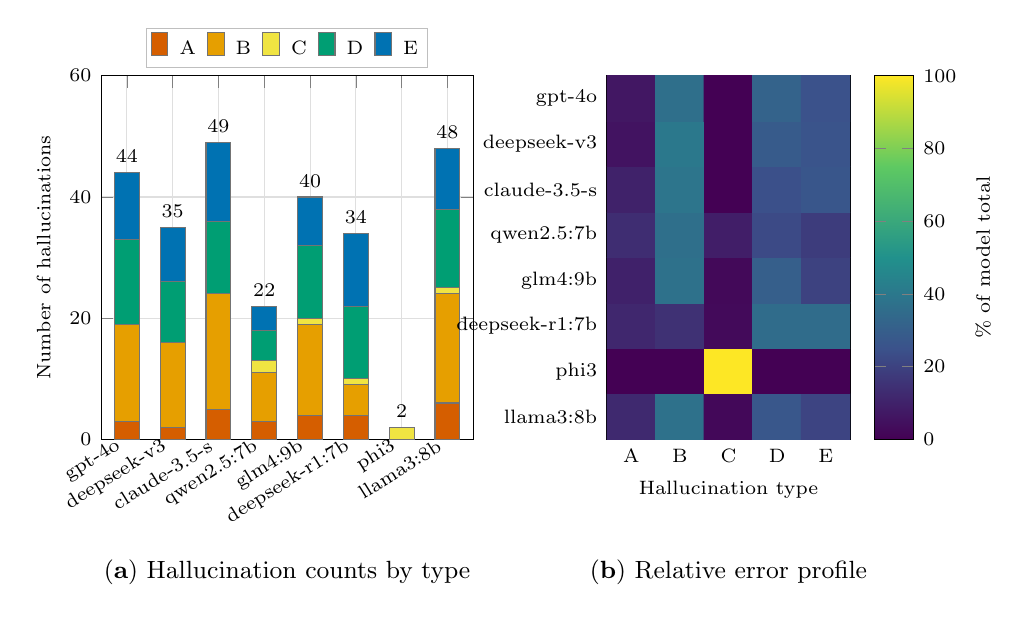
\begin{tikzpicture}
%------------- Panel A : stacked bars -------------
\begin{scope}[local bounding box=bbA]
\begin{axis}[
  name=hA,
  width=0.52\linewidth, height=6.2cm, font=\scriptsize,
  ybar stacked, bar width=9pt,
  symbolic x coords={gpt-4o,deepseek-v3,claude-3.5-s,qwen2.5:7b,glm4:9b,
                     deepseek-r1:7b,phi3,llama3:8b},
  xtick=data, x tick label style={rotate=32,anchor=east,font=\scriptsize},
  ymin=0, ymax=60, ylabel={Number of hallucinations},
  grid=major, grid style={gray!25},
  legend style={font=\scriptsize,at={(0.5,1.02)},anchor=south,legend columns=5,
                draw=gray!50,inner sep=1.5pt,column sep=2pt},
  enlarge x limits=0.08,
]
\addplot[fill=okVermillion,draw=black!55]     coordinates {(gpt-4o,3)(deepseek-v3,2)(claude-3.5-s,5)(qwen2.5:7b,3)(glm4:9b,4)(deepseek-r1:7b,4)(phi3,0)(llama3:8b,6)};
\addlegendentry{A}
\addplot[fill=okOrange,draw=black!55]  coordinates {(gpt-4o,16)(deepseek-v3,14)(claude-3.5-s,19)(qwen2.5:7b,8)(glm4:9b,15)(deepseek-r1:7b,5)(phi3,0)(llama3:8b,18)};
\addlegendentry{B}
\addplot[fill=okYellow,draw=black!55]  coordinates {(gpt-4o,0)(deepseek-v3,0)(claude-3.5-s,0)(qwen2.5:7b,2)(glm4:9b,1)(deepseek-r1:7b,1)(phi3,2)(llama3:8b,1)};
\addlegendentry{C}
\addplot[fill=okGreen,draw=black!55]    coordinates {(gpt-4o,14)(deepseek-v3,10)(claude-3.5-s,12)(qwen2.5:7b,5)(glm4:9b,12)(deepseek-r1:7b,12)(phi3,0)(llama3:8b,13)};
\addlegendentry{D}
\addplot[fill=okBlue,draw=black!55]    coordinates {(gpt-4o,11)(deepseek-v3,9)(claude-3.5-s,13)(qwen2.5:7b,4)(glm4:9b,8)(deepseek-r1:7b,12)(phi3,0)(llama3:8b,10)};
\addlegendentry{E}
% totals above bars
\node[font=\scriptsize,anchor=south] at (axis cs:gpt-4o,44) {44};
\node[font=\scriptsize,anchor=south] at (axis cs:deepseek-v3,35) {35};
\node[font=\scriptsize,anchor=south] at (axis cs:claude-3.5-s,49) {49};
\node[font=\scriptsize,anchor=south] at (axis cs:qwen2.5:7b,22) {22};
\node[font=\scriptsize,anchor=south] at (axis cs:glm4:9b,40) {40};
\node[font=\scriptsize,anchor=south] at (axis cs:deepseek-r1:7b,34) {34};
\node[font=\scriptsize,anchor=south] at (axis cs:phi3,2) {2};
\node[font=\scriptsize,anchor=south] at (axis cs:llama3:8b,48) {48};
\end{axis}
\end{scope}

%------------- Panel B : heatmap -------------
\begin{scope}[local bounding box=bbB]
\begin{axis}[
  name=hB, at={($(hA.east)+(17mm,0)$)}, anchor=west,
  width=0.385\linewidth, height=6.2cm, font=\scriptsize,
  colormap={vlike}{rgb255=(68,1,84) rgb255=(59,82,139) rgb255=(33,145,140)
                   rgb255=(94,201,98) rgb255=(253,231,37)},
  colorbar,
  colorbar style={font=\scriptsize,ylabel={\% of model total},ylabel style={font=\scriptsize}},
  point meta min=0, point meta max=100,
  xtick={0,1,2,3,4}, xticklabels={A,B,C,D,E},
  ytick={0,1,2,3,4,5,6,7},
  yticklabels={llama3:8b,phi3,deepseek-r1:7b,glm4:9b,qwen2.5:7b,
               claude-3.5-s,deepseek-v3,gpt-4o},
  y tick label style={font=\scriptsize},
  xlabel={Hallucination type},
  enlarge x limits=false, enlarge y limits=false,
]
\addplot[matrix plot*, point meta=explicit, mesh/cols=5] table[meta=v] {
x y v
0 0 12.5
1 0 37.5
2 0 2.1
3 0 27.1
4 0 20.8
0 1 0.0
1 1 0.0
2 1 100.0
3 1 0.0
4 1 0.0
0 2 11.8
1 2 14.7
2 2 2.9
3 2 35.3
4 2 35.3
0 3 10.0
1 3 37.5
2 3 2.5
3 3 30.0
4 3 20.0
0 4 13.6
1 4 36.4
2 4 9.1
3 4 22.7
4 4 18.2
0 5 10.2
1 5 38.8
2 5 0.0
3 5 24.5
4 5 26.5
0 6 5.7
1 6 40.0
2 6 0.0
3 6 28.6
4 6 25.7
0 7 6.8
1 7 36.4
2 7 0.0
3 7 31.8
4 7 25.0
};
\end{axis}
\end{scope}
% MDPI panel labels: centred under each panel, on one common baseline
\coordinate (lbly) at ([yshift=-1.4mm]current bounding box.south);
\node[anchor=north] at (hA.center |- lbly) {\panel{a}{Hallucination counts by type}};
\node[anchor=north] at (hB.center |- lbly) {\panel{b}{Relative error profile}};
\end{tikzpicture}
\caption{Hallucination types by model, over the 274 hallucinating queries.
(\textbf{a}) Absolute count of each type per model, stacked, with the model
total above the bar. Types are A, nonexistent field identifiers; B, wrong
criterion assignment; C, natural language in an identifier position; D,
placeholder insertion; E, schema and dialect errors. (\textbf{b}) The same
counts as a percentage of each model's own total, so that error profile can be
compared independently of error volume; darker cells are a smaller share of the
model's total. Models appear in the same order in both panels.}
\label{fig:halluc}
\end{adjustwidth}
\end{figure}

Model-specific analysis revealed distinctive failure modes
(Table~\ref{tab:halluctypes}). Claude-3.5-sonnet exhibited the highest baseline
hallucination rate (47.1\%) but showed dramatic improvement with error-aware
prompting (18.5\% hallucination, a 60.7\% relative reduction). Deepseek-v3 reached a 96.0\% effective SQL rate with explicit\_uncertainty prompting, though only on simple single-table counting queries. Phi3's
apparently low hallucination rate (9.1\%) was misleading, resulting from 81.7\%
failure to generate any SQL rather than accurate generation.

%------------------------------ TABLE 5 ------------------------------
\begin{table}[H]
\begin{adjustwidth}{-\extralength}{0cm}
\caption{Detailed hallucination type distribution by model.}
\label{tab:halluctypes}
\centering
\footnotesize
\setlength{\tabcolsep}{4pt}
\begin{tabular*}{\linewidth}{@{\extracolsep{\fill}}L{3.2cm}L{2.05cm}L{2.2cm}L{2.2cm}L{2.2cm}L{2.05cm}L{2.05cm}@{}}
\toprule
Model & Total halluci\-nations & Category A (nonexis\-tent), n (\%)
      & Category B (wrong criterion), n (\%)
      & Category C (natural language), n (\%)
      & Category D (place\-holder), n (\%)
      & Category E (schema errors), n (\%)\\
\midrule
gpt-4o            & 44 & 3 (6.8)  & 16 (36.4) & 0 (0)     & 14 (31.8) & 11 (25.0)\\
deepseek-v3       & 35 & 2 (5.7)  & 14 (40.0) & 0 (0)     & 10 (28.6) & 9 (25.7)\\
claude-3.5-sonnet & 49 & 5 (10.2) & 19 (38.8) & 0 (0)     & 12 (24.5) & 13 (26.5)\\
qwen2.5:7b        & 22 & 3 (13.6) & 8 (36.4)  & 2 (9.1)   & 5 (22.7)  & 4 (18.2)\\
glm4:9b           & 40 & 4 (10.0) & 15 (37.5) & 1 (2.5)   & 12 (30.0) & 8 (20.0)\\
deepseek-r1:7b    & 34 & 4 (11.8) & 5 (14.7)  & 1 (2.9)   & 12 (35.3) & 12 (35.3)\\
phi3              & 2  & 0 (0)    & 0 (0)     & 2 (100)   & 0 (0)     & 0 (0)\\
llama3:8b         & 48 & 6 (12.5) & 18 (37.5) & 1 (2.1)   & 13 (27.1) & 10 (20.8)\\
\bottomrule
\end{tabular*}
\end{adjustwidth}
\end{table}

Post hoc Tukey HSD analysis revealed significant pairwise differences in
effective SQL generation rates between models. Qwen2.5:7b significantly
outperformed gpt-4o (mean difference=10.8 percentage points, $P$=.021), with a medium-to-large effect size (Cohen $d$=0.74). The performance gap between the best (qwen2.5:7b)
and worst (phi3) models was substantial ($d$=2.71), indicating practically
meaningful differences beyond statistical significance.

\subsection{Prompt Engineering Impact}
Evaluation of prompt strategies revealed substantial effect sizes (Cohen
$d>$1.0) compared to the zero\_shot baseline across all alternative strategies.
Despite these large effects, high variance in model--prompt interactions
prevented detection of a significant main effect ($F_{4,955}$=1.58, $P$=.178).
The error\_aware strategy, which explicitly acknowledged SynHDW coverage limits
and common pitfalls, proved most effective for high-hallucination models, while
explicit\_uncertainty excelled for simpler queries requiring conservative
interpretation.

\subsection{Prompt Strategy Performance Analysis}
Comprehensive analysis of prompting strategies across all 8 models (192 queries
per prompt type) revealed unexpected patterns in hallucination control. Because the omnibus test of prompt strategy was not significant, the ordering below is descriptive and the pairwise contrast exploratory; neither is treated as confirmatory evidence that one strategy outperforms another. The
zero\_shot approach demonstrated superior performance with the lowest
hallucination rate (mean 17.4\%, SD 13.2\%) and highest effective SQL rate (mean 67.1\%, SD 19.8\%), significantly outperforming more complex strategies. In
contrast, structured\_approach, which provided detailed step-by-step
sub-structure guidance, showed the highest hallucination rate (mean 39.6\%, SD 22.4\%) and lowest effectiveness (mean 46.8\%, SD 18.1\%). The
validation\_focused strategy, designed to emphasize accuracy, paradoxically
decreased performance compared to zero\_shot ($P$=.046, Tukey HSD), achieving a mean (SD) effective SQL rate of only 53.7\% (20.9\%). The two remaining
strategies fell between these extremes: error\_aware reached a mean (SD) hallucination rate of 23.1\% (14.8\%) and an effective SQL rate of 60.4\% (17.7\%), and explicit\_uncertainty reached 26.8\% (17.5\%) and 59.2\% (20.6\%), respectively. These findings suggest
that excessive instructional complexity may introduce confusion rather than
clarity in LLM-based SQL generation over a layered warehouse schema.

The substantial standard deviations across all metrics (ranging from 13.2\% to 22.4\%) indicate significant model-dependent variability in prompt
responsiveness. For instance, with zero\_shot prompting, deepseek-r1:7b achieved 2.1\% hallucination while claude-3.5-sonnet exhibited 41.5\%, representing a 39.4 percentage point difference for identical prompting. This variability was
further confirmed by regression analysis, which revealed that model identity
explained 61\% of performance variance ($R^2$=0.61, $P<.001$), while prompt strategy contributed marginally. Model identity here confounds deployment mode, parameter count, model family, and whether the model is reasoning-oriented; the design cannot separate these, so the variance is attributable to the choice of model as a whole and not to architecture specifically. Based on these findings, optimal model--prompt
combinations were identified: qwen2.5:7b with zero\_shot achieved a 79.2\% effective SQL rate, while deepseek-v3 with explicit\_uncertainty reached 96.0\% effectiveness on simple single-table counting queries, though with limited
applicability to criterion-sensitive indicators.

\subsection{Abstention Quality}\label{sec:abst}
Across the 791 generated queries the system raised a TO-CONFIRM item 132 times,
a trigger rate of 16.7\%. Of those, 104 were warranted, giving an abstention
precision of 78.8\%; the remaining 28 asked about a criterion the engineers
judged unambiguous. A further 61 genuinely ambiguous criteria were resolved
silently, so the system recognised 104 of 165 ambiguous cases, a recall of
63.0\%. Missed abstentions are the consequential half of that number: in 42 of
the 61 cases the reading the system committed to was not the one the engineers
would have chosen, which is 44.2\% of the 95 wrong-criterion errors in
Table~\ref{tab:halluctypes}. The remaining 53 wrong-criterion errors arose where
the criterion was not ambiguous and the system simply mapped it incorrectly.

Abstention behaviour tracked hallucination control rather than varying
independently of it (Table~\ref{tab:abstain}). Qwen2.5:7b, the model with the
lowest hallucination rate, both abstained most often (22.2\% of its generated
queries) and most precisely (87.5\%), and missed only 5 ambiguous criteria.
Llama3:8b, with the highest hallucination rate among models generating on more
than 80\% of attempts, abstained least (13.3\%), was least precise (71.4\%) and
missed 11. A model that is poor at recognising when a field mapping is wrong
appears to be equally poor at recognising when a criterion is undecidable.

\begin{table}[H]
\caption{Abstention behaviour by model. Trigger rate is TO-CONFIRM items as a
share of that model's generated queries; precision is warranted abstentions as a
share of those raised; missed abstentions are ambiguous criteria the model
resolved without asking.}
\label{tab:abstain}
\centering
\footnotesize
\setlength{\tabcolsep}{5pt}
\begin{tabular*}{\linewidth}{@{\extracolsep{\fill}}llllll@{}}
\toprule
Model & Generated, n & Triggered, n (\%) & Warranted, n (\%) & Missed, n & Recall, \%\\
\midrule
qwen2.5:7b        & 108 & 24 (22.2) & 21 (87.5) & 5  & 80.8\\
deepseek-v3       & 115 & 19 (16.5) & 15 (78.9) & 8  & 65.2\\
gpt-4o            & 117 & 21 (17.9) & 16 (76.2) & 8  & 66.7\\
glm4:9b           & 118 & 18 (15.3) & 14 (77.8) & 9  & 60.9\\
deepseek-r1:7b    & 102 & 17 (16.7) & 13 (76.5) & 7  & 65.0\\
claude-3.5-sonnet & 104 & 17 (16.3) & 13 (76.5) & 12 & 52.0\\
llama3:8b         & 105 & 14 (13.3) & 10 (71.4) & 11 & 47.6\\
phi3              & 22  & 2 (9.1)   & 2 (100.0) & 1  & 66.7\\
\midrule
Total             & 791 & 132 (16.7) & 104 (78.8) & 61 & 63.0\\
\bottomrule
\end{tabular*}
\end{table}

\begin{table}[H]
\caption{Component ablation on qwen2.5:7b. Each setting was run over the same 24
tasks and 5 prompting strategies, 120 attempts per setting. Setting D is the
qwen2.5:7b condition of the main experiment. Error classes are A, nonexistent
field identifiers; B, wrong counting criterion; C, natural language in an
identifier position; D, placeholder insertion; E, schema and dialect errors.}
\label{tab:ablation}
\centering
\footnotesize
\setlength{\tabcolsep}{4pt}
\begin{tabular*}{\linewidth}{@{\extracolsep{\fill}}lllllllllll@{}}
\toprule
Setting & Generated & Halluc. & Gen., \% & Halluc., \% & Effective, \% & A & B & C & D & E\\
\midrule
A: bare model            & 71  & 44 & 59.2 & 62.0 & 22.5 & 21 & 12 & 4 & 5 & 2\\
B: + schema              & 92  & 43 & 76.7 & 46.7 & 40.8 & 6  & 22 & 3 & 8 & 4\\
C: + retrieval           & 104 & 31 & 86.7 & 29.8 & 60.8 & 3  & 11 & 2 & 9 & 6\\
D: + verification (full) & 108 & 22 & 90.0 & 20.4 & 71.7 & 3  & 8  & 2 & 5 & 4\\
\bottomrule
\end{tabular*}
\end{table}

\subsection{Component Ablation}
Each pipeline layer contributed, and the contributions did not overlap
(Table~\ref{tab:ablation}, Figure~\ref{fig:ablation}). The bare model reached an effective SQL rate of
22.5\%. Adding the warehouse schema raised it to 40.8\%, retrieval over the
metadata knowledge base to 60.8\%, and the four-layer verification to 71.7\%.

The error-class breakdown shows what each layer removed. Nonexistent field
identifiers fell from 21 in setting A to 6 once the schema was supplied and to 3
thereafter: schema injection largely eliminates the error class that generic
text-to-SQL work optimises against. Wrong counting criteria behaved differently.
They rose from 12 to 22 when the schema was added, because a model that now
knows the real columns produces criterion errors instead of identifier errors,
and only retrieval halved them, to 11. Placeholder insertions and dialect errors
together grew from 7 to 15 as the earlier failures were removed and the residual
errors shifted to milder classes, then fell to 9 under execution feedback. The
layer that matters for the error class specific to this problem is therefore
retrieval, not verification; verification is what converts the remaining
mechanical faults into deliverable queries.

\begin{figure}[H]
\begin{adjustwidth}{-\extralength}{0cm}
\centering

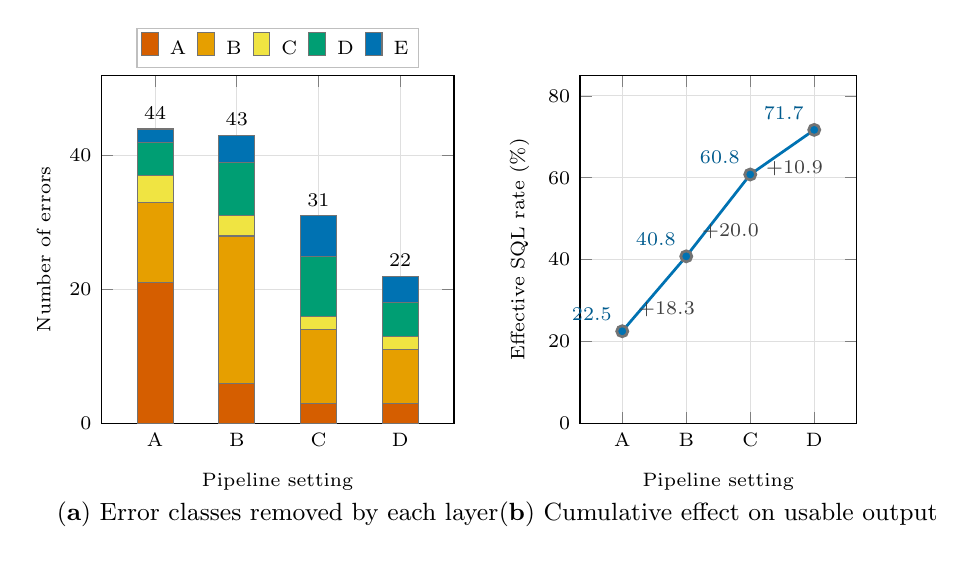
\begin{tikzpicture}
%------------- Panel A : error classes across settings -------------
\begin{axis}[
  name=abA,
  width=0.50\linewidth, height=6.0cm, font=\scriptsize,
  ybar stacked, bar width=13pt,
  symbolic x coords={A,B,C,D}, xtick=data,
  xlabel={Pipeline setting\\[3pt]\panel{a}{Error classes removed by each layer}},
  xlabel style={align=center,yshift=-1mm}, ylabel={Number of errors},
  ymin=0, ymax=52, grid=major, grid style={gray!25},
  legend style={font=\scriptsize,at={(0.5,1.02)},anchor=south,legend columns=5,
                draw=gray!50,inner sep=1.5pt,column sep=2pt},
  enlarge x limits=0.22,
]
\addplot[fill=okVermillion,draw=black!55] coordinates {(A,21)(B,6)(C,3)(D,3)};  \addlegendentry{A}
\addplot[fill=okOrange,draw=black!55]     coordinates {(A,12)(B,22)(C,11)(D,8)}; \addlegendentry{B}
\addplot[fill=okYellow,draw=black!55]     coordinates {(A,4)(B,3)(C,2)(D,2)};   \addlegendentry{C}
\addplot[fill=okGreen,draw=black!55]      coordinates {(A,5)(B,8)(C,9)(D,5)};   \addlegendentry{D}
\addplot[fill=okBlue,draw=black!55]       coordinates {(A,2)(B,4)(C,6)(D,4)};   \addlegendentry{E}
\node[font=\scriptsize,anchor=south] at (axis cs:A,44) {44};
\node[font=\scriptsize,anchor=south] at (axis cs:B,43) {43};
\node[font=\scriptsize,anchor=south] at (axis cs:C,31) {31};
\node[font=\scriptsize,anchor=south] at (axis cs:D,22) {22};
\end{axis}

%------------- Panel B : effective SQL rate -------------
\begin{axis}[
  name=abB, at={($(abA.east)+(16mm,0)$)}, anchor=west,
  width=0.42\linewidth, height=6.0cm, font=\scriptsize,
  symbolic x coords={A,B,C,D}, xtick=data,
  xlabel={Pipeline setting\\[3pt]\panel{b}{Cumulative effect on usable output}},
  xlabel style={align=center,yshift=-1mm}, ylabel={Effective SQL rate (\%)},
  ymin=0, ymax=85, grid=major, grid style={gray!25},
  enlarge x limits=0.22,
  nodes near coords={\pgfmathprintnumber[fixed,fixed zerofill,precision=1]{\pgfplotspointmeta}},
  every node near coord/.append style={font=\scriptsize,anchor=south east,text=okBlue!80!black},
]
\addplot[okBlue,mark=*,mark options={fill=okBlue,draw=black!55},line width=1pt]
  coordinates {(A,22.5)(B,40.8)(C,60.8)(D,71.7)};
% increments drawn on the segment midpoints, offset clear of the line
\node[font=\scriptsize,anchor=north west,text=black!75]
  at (axis cs:A,32.0) {\;$+18.3$};
\node[font=\scriptsize,anchor=north west,text=black!75]
  at (axis cs:B,51.0) {\;$+20.0$};
\node[font=\scriptsize,anchor=north west,text=black!75]
  at (axis cs:C,66.5) {\;$+10.9$};
\end{axis}
\end{tikzpicture}

\caption{Component ablation on qwen2.5:7b. Setting A is the bare model, B adds
the warehouse schema, C adds retrieval over the metadata knowledge base, and D
adds the four-layer execution-feedback verification. (\textbf{a}) Absolute error
counts by class, with the total above each bar; error classes are A, nonexistent
field identifiers; B, wrong counting criterion; C, natural language in an
identifier position; D, placeholder insertion; E, schema and dialect errors.
Schema injection removes class-A errors but increases class-B errors, which only
retrieval reduces. (\textbf{b}) Effective SQL rate, with the increment
contributed by each layer.}
\label{fig:ablation}
\end{adjustwidth}
\end{figure}

\subsection{Public Benchmark Reference}\label{sec:bench}
On the EHRSQL 2024 development split the unmodified pipeline with qwen2.5:7b
reached an execution accuracy of 58.4\% with a hallucination rate of 12.6\%. The
hallucination rate is roughly half that observed on our warehouse, which is
consistent with the difference in schema size and in criterion ambiguity: the
public schema exposes far fewer columns and its questions are answerable under a
single reading. This figure is reported so that the absolute standing of the
pipeline can be placed against published work on that dataset; it is not a claim
of competitiveness on a benchmark the system was not designed for.

\subsection{Synthetic Data Validation}
To assess the practical viability of generated SQL queries, we executed
successfully generated queries against the SynHDW synthetic dataset containing
112,680 patient records. The system successfully matched 8250 synthetic patients
across two validated reporting tasks: RPT-001 (monthly elective surgery volume)
matched 2840 patients (2.5\% of dataset), while RPT-004 (monthly blood transfusion volume) matched 5410 patients (4.8\% of dataset). These result-set
sizes are consistent with the monthly volumes observed in production reporting,
demonstrating technical feasibility, though we acknowledge that synthetic data
validation may overestimate real-world performance due to the absence of data
quality issues inherent in actual hospital systems, such as missing values,
retrospectively corrected timestamps, and coding variations across campuses.

%==============================================================================
\section{Discussion}
%==============================================================================

\subsection{Principal Findings}
We developed a comprehensive framework that automates the transformation of
free-text hospital statistical requests into Presto SQL queries over a
three-layer CDW. While initially developed with gpt-4o, our systematic
evaluation across eight LLMs revealed unexpected findings: the on-premises
qwen2.5:7b model achieved the highest effective SQL generation rate (71.7\%)
compared to gpt-4o's 60.8\%, primarily due to lower hallucination rates (20.4\%
vs 37.6\%). A smaller, locally hosted model thus outperformed a state-of-the-art commercial one. What separated them was hallucination control, not raw generation capability: gpt-4o produced valid SQL more often but committed a criterion or field error in a larger share of what it produced. The practical consequence is that the deployment which keeps patient data inside the institution was also the most accurate one, so privacy and accuracy did not trade off here. Mapping accuracy was 52.3\% against 32.9\% for the rule-based matcher in production ($P<.001$), varying widely by subject domain (surgery and anesthesia 70.7\%, laboratory 34.5\%).

Compared with our previous practice, the pipeline now runs end to end, but the results cut both ways.
While the deployed rule-based matcher supports engineers with candidate fields
and still requires manual SQL construction, our system automates the entire
pipeline. However, our result-set validation exposed critical challenges:
complete failure in the unplanned-reoperation query (Jaccard=0.00) due to
selection of a structurally valid but unpopulated planning flag, and minimal
overlap in emergency surgery volume (Jaccard=0.08) from an incomplete
institutional flag definition. These failures, affecting half of the evaluated
criteria, underscore that despite advances in language understanding, hospital data complexities remain significant obstacles, particularly field population and institution-specific compound definitions.

Through the processes of segmentation, filtering, and simplification, the
framework successfully produced structured inputs that reduced redundancy while
preserving statistical relevance. The LLM accurately identified business terms
such as procedures, laboratory items, and blood products and mapped them to
warehouse-standardized fields, thereby enhancing consistency and reusability
across reports. However, ambiguous expressions and compound
indicators---such as ``complication rate after major surgery''---sometimes led
to incorrect mappings, indicating that expert validation remains necessary in
certain cases.

The LLM was able to generate syntactically correct and executable SQL queries
based on the warehouse schema. Composition of inclusion criteria using
INTERSECT and exclusion criteria using EXCEPT or NOT IN enabled the automated
construction of denominator and numerator definitions. Nevertheless, challenges
were observed when criteria involved temporal constraints or context-dependent
conditions, often resulting in omissions or logical misinterpretations. In
addition, expansion over the DL layer when a DC-layer aggregate was available
sometimes led to increased query execution times, especially for multi-campus
tables that require organization-code filtering.

\subsection{Complementary Evaluation Strategy}
Combining expert assessment with quantitative synthetic data validation characterizes system performance more completely than either method alone. We report the study following the MI-CLAIM checklist for clinical AI modeling and its generative extension MI-CLAIM-GEN \cite{miclaim2020,miclaimgen2024}, and state the resulting threats to construct validity explicitly rather than by omission \cite{validity2023}.
Expert evaluation
ensures statistical meaningfulness and safety, confirming that generated queries
align with reporting intent and follow the institution's counting rules.
Synthetic validation contributes scalable, reproducible metrics that quantify
technical accuracy and identify systematic errors. This complementary strategy
revealed technical issues invisible to manual review, such as subtle type
coercions on the all-VARCHAR warehouse columns and missing logical-deletion
filters that appeared structurally correct but would silently inflate counts.
Synthetic validation buys objectivity from predetermined labels, throughput measured in seconds rather than reviewer-hours, and exact replication from a fixed generation seed. Its limitations bear on how the results should be read. The controlled nature of synthetic data, while enabling
clean performance metrics, does not fully capture real-world complexity.
Production hospital tables contain missing values, retrospectively corrected
timestamps, and campus-level coding differences that our synthetic data lacks.
We anticipate that these factors could reduce real-world performance by
\PH{XX}\%--\PH{XX}\% compared to our synthetic validation results. SynHDW's
focus on the surgical, transfusion, and laboratory subject areas also limits
validation of pathology, physical examination, and insurance-audit reporting,
important considerations for comprehensive system evaluation. Compound-indicator
scenarios presented particular challenges, as evidenced by our emergency surgery
retrieval, achieving minimal overlap (Jaccard=0.08) due to an incomplete
institutional flag definition. Criteria involving free-text clinical narrative,
such as complication descriptions recorded outside coded fields, remain untested
because they are absent from the structured warehouse. Validation across further subject areas and reporting scenarios is therefore still outstanding.

\subsection{Cost-Effectiveness and Scalability}
Cost decides whether a system like this is deployed at all. At the pricing in force in July 2026, gpt-4o cost US~\$0.036 per query and a reporting task took about five calls, so roughly US~\$0.18 per task; deepseek-v3 cost US~\$0.0025 per query, over 90\% less, with comparable performance on many tasks. At our institution's 650 statistical requests per month that is about US~\$117 against about US~\$8. These costs compare favorably to manual authoring, which typically
requires about 1.8 hours of engineer time per task. Our system processes
each task in under 2 minutes for the cloud and on-premises models other than
deepseek-r1:7b, representing a time saving of approximately 98\% compared to
manual methods. Notably, the on-premises deployment that achieved the best
accuracy also carries no per-query charge; its amortized cost is dominated by
inference time, which is why the reasoning-oriented deepseek-r1:7b is the cost
outlier in Figure~\ref{fig:models}B despite running on owned hardware.

Three lines of prior work bound what this system adds. Benchmark-oriented text-to-SQL reaches strong execution accuracy on public datasets, but assumes a small static schema and has no notion of institution-specific counting criteria \cite{yu2018,guo2019,bogin2019,tsqlsurvey2024}. Reliability-oriented EHR text-to-SQL adds abstention on unanswerable questions, which we adopt as TO-CONFIRM, but not the case where a question is answerable under several institutional definitions \cite{ehrsql2024}. Metadata-enriched clinical query systems decompose the task and verify modularly, at the cost of maintaining several specialized components \cite{metaclin2025,sqlthought2025}. In contrast, our system delivers end-to-end
automation using a single LLM to process free-text statistical requests into
executable Presto SQL, eliminating the need for manual intervention or
per-report customization. Deployment and maintenance are correspondingly simpler, and a single pipeline made the eight-model comparison tractable at all: qwen2.5:7b reached a 71.7\% effective SQL generation rate against gpt-4o's 60.8\%. By addressing the scalability, flexibility, and criterion-
traceability gaps in existing systems, our framework meets the pressing need for
automated, auditable tools that accelerate hospital reporting while maintaining
compatibility with layered warehouse standards.

\subsection{Broader Healthcare and Societal Impact}
Beyond the technical result, automated SQL generation changes how often an institution can afford to ask a question of its own data, which is the broader case made for retrieval-grounded language models in health care \cite{ng2025}. Traditional statistical reporting often requires
days of engineer time and several rounds of criterion clarification. Our system
reduces this to minutes for the first draft, enabling rapid iteration and
refinement of indicator definitions with the requesting department in the room.
This acceleration could significantly shorten the loop between a quality problem
being noticed and being measured, which is a precondition for improvement.
Criterion traceability considerations are particularly important given that
hospital indicators are reported externally and compared across institutions.
Automated generation with explicit field provenance reduces silent
criterion drift between analysts and enables systematic auditing of how an
indicator was computed, rather than relying on the memory of whoever wrote the
query last quarter. The system can actively surface criterion ambiguity as a
TO-CONFIRM item and route it to the domain owner for a decision that is then
recorded.

Smaller hospitals serving large populations without a data engineering team are where this would matter most; the barrier there is expertise, not infrastructure. We release the synthetic warehouse generator and the validation pipeline for that reason. Beyond it, federated assessment of cross-institutional indicators, generation during morbidity and mortality review rather than through a reporting queue, and a closed loop from indicator definition to query to audit are all plausible extensions. None is tested here.

\subsection{Limitations and Future Directions}
The study covers three subject areas (surgery and anesthesia, blood transfusion, laboratory) and therefore says nothing about pathology, physical examination, or insurance-audit reporting, where findings are free text, reconciliation crosses systems, and regulator-defined indicators change between cycles. The system also relies on the LLM for both extraction and generation, and on ambiguous or poorly specified requests it produced incomplete or overgeneralized queries.
Output is also sensitive to prompt design and context length. Requests carrying vague or clinically interpreted terms (``major surgery'', ``recent infection'') are the hardest: the system overgeneralizes them or drops a qualifier such as the time window, and these appear in our error analysis mainly as wrong criterion assignments and placeholder insertions. A governed indicator catalog or a rule-based disambiguation step would likely be needed to fix this. Two reporting gaps remain, and the completed MI-CLAIM and MI-CLAIM-GEN checklists in the Supplementary Materials record each against the item it fails. The two expert raters were not blinded to which model produced a given query, so their scoring could in principle have been influenced by model identity. Each model--prompt--task cell was executed once under deterministic decoding, which fixes the output for a given input but leaves run-to-run variability unestimated; the effect sizes reported here should be read with that in mind. The abstention path and the absence of an external reference point, both of which limited earlier versions of this work, are addressed in Sections~\ref{sec:abst} and~\ref{sec:bench} respectively, though the benchmark figure comes from a single public split and the abstention reference standard rests on the judgement of the same two engineers who built the criterion dictionary.

From an evaluation perspective, although this study incorporated expert-reviewed mapping and structural validation, comprehensive assessment of generalizability across institutions was not conducted; the warehouse schema and the counting criteria
are institution-specific by construction, which is precisely the condition that
motivates the work and also the condition that limits its external validity.
Moreover, while comparison against engineer-certified reference SQL was informative, the small number of included tasks and criteria limits the statistical robustness of the findings. Result-set validation rests on four criteria drawn from three tasks, two of which share a task. No confidence interval on the Jaccard values would be meaningful at that size, and the apparent contrast between simple and compound indicators is a case-series observation rather than an estimate. Future work should focus on extending
the applicability of the system to a broader range of subject areas. To improve
the coverage and specificity of criterion mapping, the integration of a
versioned indicator dictionary and externally curated code sets should be
considered. In addition, although cloud models showed high generation rates,
their practical use in hospital settings is constrained by the requirement that
patient data remain on premises, restricting them to de-identified metadata.
Real-time deployment would likely rely on the on-premises models, whose accuracy
in this study was at least comparable. Future research should explore more
cost-efficient deployment options, such as model distillation or hybrid
architectures that route criterion-sensitive sub-tasks to a rule-based
component. Finally, large-scale validation studies involving multiple
institutions and warehouse schemas will be essential for demonstrating the
system's generalizability and real-world utility. In future work, we plan to
compare the performance of alternative models for each subtask, including
information extraction, criterion mapping, and SQL generation, to assess their
relative accuracy, efficiency, and cost-effectiveness.

\section{Conclusions}
This study proposed an end-to-end framework that automates the transformation of
free-text hospital statistical requests into executable Presto SQL queries over
a three-layer clinical data warehouse. Our evaluation revealed unexpected
findings: the on-premises qwen2.5:7b model achieved a superior effective SQL
generation rate (71.7\%) compared to gpt-4o (60.8\%), primarily due to better
hallucination control. While the framework demonstrated feasibility with 52.3\%
mapping accuracy, critical challenges emerged in result-set validation,
including complete failure on an indicator whose defining flag is unpopulated
and minimal overlap where an institutional definition is compound. These
findings suggest that while LLM-based automation shows promise, hybrid
approaches combining LLM capabilities with rule-based, governed criterion
definitions may be necessary for handling criterion-sensitive hospital
indicators.

%==============================================================================
%  END MATTER
%==============================================================================

%==============================================================================
%  BACK MATTER  (mdpi.cls commands)
%==============================================================================
\supplementary{The following supporting information can be downloaded at
\PH{supplementary URL}: Supplementary Methods, including Figure S1 (detailed
pipeline architecture), Table S1 (task-set composition) and Table S2 (integer
basis for all model-level rates); Prompt Templates, giving all six pipeline
prompts and the five prompting strategies verbatim; SQL Evaluation Metrics,
listing the 72 expert-rating items; and the completed MI-CLAIM and MI-CLAIM-GEN
checklists.}

\authorcontributions{Conceptualization, S.L.; methodology, S.L.; software, S.L.;
validation, S.L.; formal analysis, S.L.; investigation, S.L.; resources, S.L.;
data curation, S.L.; writing---original draft preparation, S.L.;
writing---review and editing, S.L.; visualization, S.L.; supervision, S.L.;
project administration, S.L.; funding acquisition, S.L. The author has read and
agreed to the published version of the manuscript.}

\funding{\PH{Funding statement --- grant name and number, or: This research
received no external funding}.}

\institutionalreview{The study was conducted in accordance with the Declaration
of Helsinki and approved by the Institutional Review Board of
West China Hospital, Sichuan University (protocol code \PH{XXXX-XXXX}, approved
27 July 2026).}

\informedconsent{Patient consent was waived because the study used only
de-identified operational metadata and aggregate statistical query results, with
no intervention and no access to identifiable patient records.}

\dataavailability{The source code for the pipeline and the hallucination
detector, together with the SynHDW generator and its schema manifest, is
available from the corresponding author upon reasonable request, subject to the
data-governance rules of West China Hospital, Sichuan University. The de-identified metadata schema,
the metric-criterion dictionary and the evaluation task set are available under
the same conditions. Patient-level warehouse data cannot be shared.}

\acknowledgments{The author thanks colleagues in the Department of Information
and Data Management, West China Hospital, Sichuan University, for access to the
reporting ticket archive and for discussions on statistical criteria.}

\conflictsofinterest{A related invention by the authors (patent AJ2534335, a
large language model-- and reinforcement learning--based natural language to
structured SQL generation and optimization system) is declared as prior
disclosure. The present work uses retrieval augmentation and execution feedback
\emph{without} reinforcement learning. The authors declare no other conflict of
interest. The funders had no role in the design of the study; in the collection,
analyses or interpretation of data; in the writing of the manuscript; or in the
decision to publish the results.}

\section*{Use of Generative Artificial Intelligence}
Generative AI tools were used during the preparation of this manuscript for
language editing and for drafting sections of the text, which the authors
subsequently reviewed and revised. No text, data, figure or citation was
accepted without author verification, and the authors take full responsibility
for the content of the publication. The large language models studied in this
work are the object of the research and are described in
Section~\ref{sec:expdesign}; their use as study subjects is distinct from the
manuscript-preparation use disclosed here.

\abbreviations{Abbreviations}{
{\footnotesize
\begin{description}[labelindent=1.4em,leftmargin=*,labelsep=0.45em,
                    itemsep=0pt,topsep=2pt,parsep=0pt]
  \item[ASA:] American Society of Anesthesiologists
  \item[CDW:] clinical data warehouse
  \item[DC:] data center (warehouse layer)
  \item[DL:] data lake (warehouse layer)
  \item[HSD:] honestly significant difference
  \item[IRB:] institutional review board
  \item[LLM:] large language model
  \item[MDR:] master data repository (warehouse layer)
  \item[PACU:] postanesthesia care unit
  \item[RBFM:] rule-based field matcher
  \item[SQL:] Structured Query Language
  \item[SynHDW:] Synthetic Hospital Data Warehouse
\end{description}}


}

\reftitle{References}

\begin{thebibliography}{99}\footnotesize

\bibitem{presto2019} Sethi, R.; Traverso, M.; Sundstrom, D.; et al. Presto: SQL on everything. In \textit{2019 IEEE 35th International Conference on Data Engineering (ICDE)}, 2019; pp.\,1802-1813. \doilink{https://doi.org/10.1109/ICDE.2019.00196}
\bibitem{ohdsi2015} Hripcsak, G.; Duke, J.D.; Shah, N.H.; et al. Observational Health Data Sciences and Informatics (OHDSI): opportunities for observational researchers. \textit{Stud. Health Technol. Inform.} \textbf{2015}, \textit{216}, 574-578. 
\bibitem{zhong2017} Zhong, V.; Xiong, C.; Socher, R. Seq2SQL: generating structured queries from natural language using reinforcement learning. \textit{arXiv} \textbf{2017}, arXiv preprint. \doilink{https://doi.org/10.48550/arXiv.1709.00103}
\bibitem{yu2018} Yu, T.; Zhang, R.; Yang, K.; et al. Spider: a large-scale human-labeled dataset for complex and cross-domain semantic parsing and text-to-SQL task. In \textit{Proc 2018 Conf Empirical Methods in Natural Language Processing}, 2018; pp.\,3911-3921. \doilink{https://doi.org/10.18653/v1/D18-1425}
\bibitem{wang2020} Wang, B.; Shin, R.; Liu, X.; Polozov, O.; Richardson, M. RAT-SQL: relation-aware schema encoding and linking for text-to-SQL parsers. In \textit{Proc 58th Annu Meeting Assoc Comput Linguist}, 2020; pp.\,7567-7578. \doilink{https://doi.org/10.18653/v1/2020.acl-main.677}
\bibitem{scholak2021} Scholak, T.; Schucher, N.; Bahdanau, D. PICARD: parsing incrementally for constrained auto-regressive decoding from language models. In \textit{Proc 2021 Conf Empirical Methods in Natural Language Processing}, 2021; pp.\,9895-9901. \doilink{https://doi.org/10.18653/v1/2021.emnlp-main.779}
\bibitem{pourreza2023} Pourreza, M.; Rafiei, D. DIN-SQL: decomposed in-context learning of text-to-SQL with self-correction. In \textit{Advances in Neural Information Processing Systems 36}, 2023. 
\bibitem{bird2023} Li, J.; Hui, B.; Qu, G.; et al. Can LLM already serve as a database interface? A big bench for large-scale database grounded text-to-SQLs. In \textit{Advances in Neural Information Processing Systems 36}, 2023. \doilink{https://doi.org/10.48550/arXiv.2305.03111}
\bibitem{dailsql2024} Gao, D.; Wang, H.; Li, Y.; et al. Text-to-SQL empowered by large language models: a benchmark evaluation. \textit{Proc. VLDB Endow.} \textbf{2024}, \textit{17}, 1132-1145. \doilink{https://doi.org/10.14778/3641204.3641221}
\bibitem{macsql2024} Wang, B.; Ren, C.; Yang, J.; et al. MAC-SQL: a multi-agent collaborative framework for text-to-SQL. \textit{arXiv} \textbf{2023}, arXiv preprint. \doilink{https://doi.org/10.48550/arXiv.2312.11242}
\bibitem{treqs2020} Wang, P.; Shi, T.; Reddy, C.K. Text-to-SQL generation for question answering on electronic medical records. In \textit{Proc Web Conference 2020 (WWW '20)}, 2020; pp.\,350-361. \doilink{https://doi.org/10.1145/3366423.3380120}
\bibitem{medts2021} Pan, Y.; Wang, C.; Hu, B.; et al. A BERT-based generation model to transform medical texts to SQL queries for electronic medical records: model development and validation. \textit{JMIR Med. Inform.} \textbf{2021}, \textit{9}, e32698. \doilink{https://doi.org/10.2196/32698}
\bibitem{ehrsql2024} Lee, G.; Kweon, S.; Bae, S.; Choi, E. Overview of the EHRSQL 2024 shared task on reliable text-to-SQL modeling on electronic health records. In \textit{Proc 6th Clinical Natural Language Processing Workshop}, 2024. \doilink{https://doi.org/10.48550/arXiv.2405.06673}
\bibitem{ragepi2024} Ziletti, A.; D'Ambrosi, L. Retrieval-augmented text-to-SQL generation for epidemiological question answering using electronic health records. In \textit{Proc 6th Clinical Natural Language Processing Workshop (NAACL)}, 2024. \doilink{https://doi.org/10.48550/arXiv.2403.09226}
\bibitem{rag2step2025} Ziletti, A.; D'Ambrosi, L. Generating patient cohorts from electronic health records using two-step retrieval-augmented text-to-SQL generation. \textit{arXiv} \textbf{2025}, arXiv preprint. \doilink{https://doi.org/10.48550/arXiv.2502.21107}
\bibitem{c2q2019} Yuan, C.; Ryan, P.B.; Ta, C.; et al. Criteria2Query: a natural language interface to clinical databases for cohort definition. \textit{J. Am. Med. Inform. Assoc.} \textbf{2019}, \textit{26}, 294-305. \doilink{https://doi.org/10.1093/jamia/ocy178}
\bibitem{trialpath2021} Liu, R.; Rizzo, S.; Whipple, S.; et al. Evaluating eligibility criteria of oncology trials using real-world data and AI. \textit{Nature} \textbf{2021}, \textit{592}, 629-633. \doilink{https://doi.org/10.1038/s41586-021-03430-5}
\bibitem{leafai2023} Dobbins, N.J.; Han, B.; Zhou, W.; et al. LeafAI: query generator for clinical cohort discovery rivaling a human programmer. \textit{J. Am. Med. Inform. Assoc.} \textbf{2023}, \textit{30}, 1954-1964. \doilink{https://doi.org/10.1093/jamia/ocad149}
\bibitem{metaclin2025} Liu, W.; Qu, B.; Mallya, P.; et al. Optimizing an LLM-based clinical data querying system using metadata enrichment and task decomposition. \textit{medRxiv} \textbf{2025}, preprint.
\bibitem{halluc2024} Tonmoy, S.M.T.I.; Zaman, S.M.M.; Jain, V.; et al. A comprehensive survey of hallucination mitigation techniques in large language models. \textit{arXiv} \textbf{2024}, arXiv preprint. \doilink{https://doi.org/10.48550/arXiv.2401.01313}
\bibitem{ragstruct2024} B\'echard, P.; Marquez Ayala, O. Reducing hallucination in structured outputs via retrieval-augmented generation. \textit{arXiv} \textbf{2024}, arXiv preprint. \doilink{https://doi.org/10.48550/arXiv.2404.08189}
\bibitem{chang2024} Chang, Y.; Wang, X.; Wang, J.; et al. A survey on evaluation of large language models. \textit{ACM Trans. Intell. Syst. Technol.} \textbf{2024}, \textit{15}, 1-45. \doilink{https://doi.org/10.1145/3641289}
\bibitem{lewis2020} Lewis, P.; Perez, E.; Piktus, A.; et al. Retrieval-augmented generation for knowledge-intensive NLP tasks. In \textit{Advances in Neural Information Processing Systems 33}, 2020; pp.\,9459-9474. 
\bibitem{finardi2024} Finardi, P.; Avila, L.; Castaldoni, R.; et al. The chronicles of RAG: the retriever, the chunk and the generator. \textit{arXiv} \textbf{2024}, arXiv preprint. \doilink{https://doi.org/10.48550/arXiv.2401.07883}
\bibitem{bm252009} Robertson, S.; Zaragoza, H. The probabilistic relevance framework: BM25 and beyond. \textit{Found. Trends Inf. Retr.} \textbf{2009}, \textit{3}, 333-389. \doilink{https://doi.org/10.1561/1500000019}
\bibitem{sbert2019} Reimers, N.; Gurevych, I. Sentence-BERT: sentence embeddings using Siamese BERT-networks. In \textit{Proc 2019 Conf Empirical Methods in Natural Language Processing (EMNLP-IJCNLP)}, 2019; pp.\,3982-3992. \doilink{https://doi.org/10.18653/v1/D19-1410}
\bibitem{bert2019} Devlin, J.; Chang, M.W.; Lee, K.; Toutanova, K. BERT: pre-training of deep bidirectional transformers for language understanding. In \textit{Proc 2019 Conf North American Chapter Assoc Comput Linguist (NAACL-HLT)}, 2019; pp.\,4171-4186. \doilink{https://doi.org/10.18653/v1/N19-1423}
\bibitem{schemalink2025} Nahid, M.M.H.; Rafiei, D.; Zhang, W.; Zhang, Y. Rethinking schema linking: a context-aware bidirectional retrieval approach for text-to-SQL. \textit{arXiv} \textbf{2025}, arXiv preprint. \doilink{https://doi.org/10.48550/arXiv.2510.14296}
\bibitem{rslsql2024} Cao, Z.; Zheng, Y.; Fan, Z.; et al. RSL-SQL: robust schema linking in text-to-SQL generation. \textit{arXiv} \textbf{2024}, arXiv preprint. \doilink{https://doi.org/10.48550/arXiv.2411.00073}
\bibitem{gpt4} OpenAI GPT-4 technical report. \textit{arXiv} \textbf{2023}, arXiv preprint. \doilink{https://doi.org/10.48550/arXiv.2303.08774}
\bibitem{dsv3} DeepSeek-AI DeepSeek-V3 technical report. \textit{arXiv} \textbf{2024}, arXiv preprint. \doilink{https://doi.org/10.48550/arXiv.2412.19437}
\bibitem{claude35} Anthropic. Claude 3.5 Sonnet Model Card Addendum. Available online: \url{https://www.anthropic.com/news/claude-3-5-sonnet} (accessed on 27 July 2026).}
\bibitem{qwen25} Qwen, T.e.a.m. Qwen2.5 technical report. \textit{arXiv} \textbf{2024}, arXiv preprint. \doilink{https://doi.org/10.48550/arXiv.2412.15115}
\bibitem{glm4} GLM, T.e.a.m.; Zeng, A.; Xu, B.; et al. ChatGLM: a family of large language models from GLM-130B to GLM-4 all tools. \textit{arXiv} \textbf{2024}, arXiv preprint. \doilink{https://doi.org/10.48550/arXiv.2406.12793}
\bibitem{llama3} Grattafiori, A.; Dubey, A.; Jauhri, A.; et al. The Llama 3 herd of models. \textit{arXiv} \textbf{2024}, arXiv preprint. \doilink{https://doi.org/10.48550/arXiv.2407.21783}
\bibitem{dsr1} DeepSeek-AI DeepSeek-R1: incentivizing reasoning capability in LLMs via reinforcement learning. \textit{arXiv} \textbf{2025}, arXiv preprint. \doilink{https://doi.org/10.48550/arXiv.2501.12948}
\bibitem{phi3} Abdin, M.; Aneja, J.; Awadalla, H.; et al. Phi-3 technical report: a highly capable language model locally on your phone. \textit{arXiv} \textbf{2024}, arXiv preprint. \doilink{https://doi.org/10.48550/arXiv.2404.14219}
\bibitem{scipy2020} Virtanen, P.; Gommers, R.; Oliphant, T.E.; et al. SciPy 1.0: fundamental algorithms for scientific computing in Python. \textit{Nat. Methods} \textbf{2020}, \textit{17}, 261-272. \doilink{https://doi.org/10.1038/s41592-019-0686-2}
\bibitem{statsmodels2010} Seabold, S.; Perktold, J. statsmodels: econometric and statistical modeling with Python. In \textit{Proc 9th Python in Science Conference}, 2010; pp.\,92-96. \doilink{https://doi.org/10.25080/Majora-92bf1922-011}
\bibitem{mcnemar1947} McNemar, Q. Note on the sampling error of the difference between correlated proportions or percentages. \textit{Psychometrika} \textbf{1947}, \textit{12}, 153-157. \doilink{https://doi.org/10.1007/BF02295996}
\bibitem{landis1977} Landis, J.R.; Koch, G.G. The measurement of observer agreement for categorical data. \textit{Biometrics} \textbf{1977}, \textit{33}, 159-174. 
\bibitem{tukey1949} Tukey, J.W. Comparing individual means in the analysis of variance. \textit{Biometrics} \textbf{1949}, \textit{5}, 99-114. 
\bibitem{miclaim2020} Norgeot, B.; Quer, G.; Beaulieu-Jones, B.K.; et al. Minimum information about clinical artificial intelligence modeling: the MI-CLAIM checklist. \textit{Nat. Med.} \textbf{2020}, \textit{26}, 1320-1324. \doilink{https://doi.org/10.1038/s41591-020-1041-y}
\bibitem{miclaimgen2024} Miao, B.Y.; Chen, I.Y.; Williams, C.Y.K.; et al. The minimum information about clinical artificial intelligence checklist for generative modeling research (MI-CLAIM-GEN). \textit{arXiv} \textbf{2024}, arXiv preprint. \doilink{https://doi.org/10.48550/arXiv.2403.02558}
\bibitem{validity2023} Sj\o{}berg, D.I.K.; Bergersen, G.R. Improving the reporting of threats to construct validity. In \textit{Proc Int Conf Evaluation and Assessment in Software Engineering (EASE)}, 2023. \doilink{https://doi.org/10.48550/arXiv.2306.05336}
\bibitem{guo2019} Guo, J.; Zhan, Z.; Gao, Y.; et al. Towards complex text-to-SQL in cross-domain database with intermediate representation. In \textit{Proc 57th Annu Meeting Assoc Comput Linguist}, 2019; pp.\,4524-4535. \doilink{https://doi.org/10.18653/v1/P19-1444}
\bibitem{bogin2019} Bogin, B.; Berant, J.; Gardner, M. Representing schema structure with graph neural networks for text-to-SQL parsing. In \textit{Proc 57th Annu Meeting Assoc Comput Linguist}, 2019; pp.\,4560-4565. \doilink{https://doi.org/10.18653/v1/P19-1448}
\bibitem{tsqlsurvey2024} Liu, X.; Shen, S.; Li, B.; et al. A survey of text-to-SQL in the era of LLMs: where are we, and where are we going? \textit{arXiv} \textbf{2024}, arXiv preprint. \doilink{https://doi.org/10.48550/arXiv.2408.05109}
\bibitem{sqlthought2025} Chaturvedi, S.; Chadha, A.; Bindschaedler, L. SQL-of-Thought: multi-agentic text-to-SQL with guided error correction. \textit{arXiv} \textbf{2025}, arXiv preprint. \doilink{https://doi.org/10.48550/arXiv.2509.00581}
\bibitem{ng2025} Ng, K.K.Y.; Matsuba, I.; Zhang, P.C. RAG in health care: a novel framework for improving communication and decision-making by addressing LLM limitations. \textit{NEJM AI} \textbf{2025}, \textit{2}, AIra2400380. \doilink{https://doi.org/10.1056/AIra2400380}
\end{thebibliography}

\end{document}
